\chapter{Validation}
\label{chp:validation}
% Probably the biggest chapter:
% - explain the metrics
% - explain the scenarios
% - display the good and bad results (highlight both)
% - display the high level results

% Why is validation needed?
Now that the prototype has been build, it needs to be evaluated to assess the accuracy of the implemented algorithms. This chapter goes into depth about the validation methods and the validation results.

\section{Variables used}
To validate this project correctly, the variables that are worked with must be established. With these variables in mind, some can be changed while others remain the same. In this way, it can be determined which variable has an impact on the accuracy of the sensor. 

\subsection{Recorded variables}
The recorded variables are the measurements that are being taken to measure the vital signs for a person. These measurements are coming from the sensor, but also from other devices to validate the measurements from the sensor. The sensor itself measures the heart rate and respiration rate from one or multiple persons. But not only this information gets send back to the computer. To make the visualization on the computer a bit better, different waveforms are also send to the computer. There is one unfiltered waveform, a heart rate waveform and a respiration rate waveform. The unfiltered waveform is the phase of the radar data for the bin in which the measured person is residing. The heart rate and respiration rate waveforms are the waveforms from which the heart rate and respiration rate can be determined. These waveforms are being generated after the filtering of the phase signal, see also Section~\ref{sec:vit_signs_est}. For a snapshot of the GUI on the computer, see Figure~\ref{fig:gui_computer}.

\begin{figure}[ht]
    \centering
    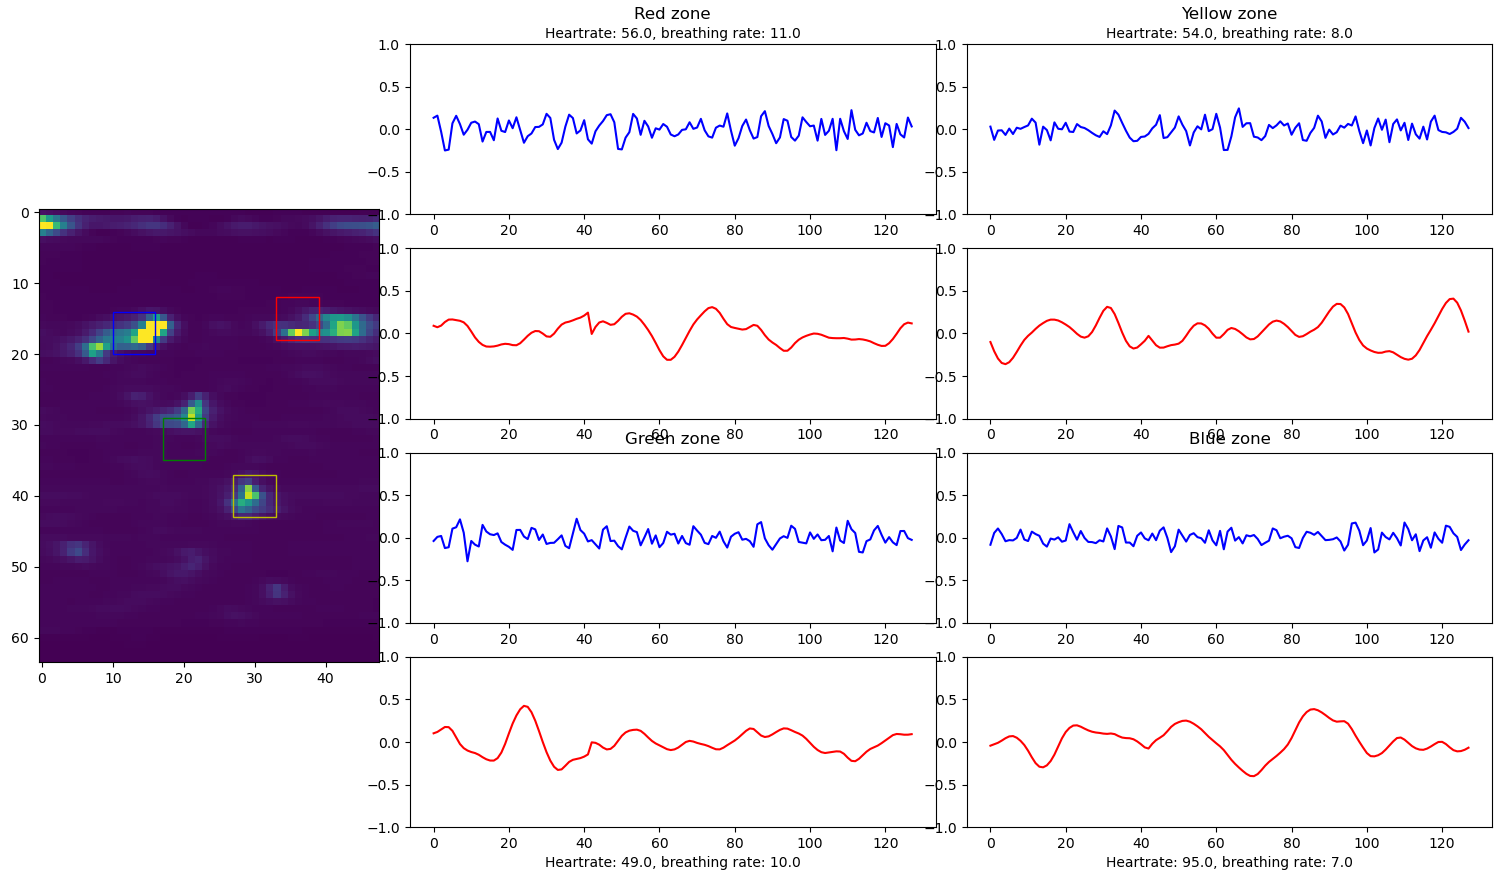
\includegraphics[width=.95\textwidth]{figures/validation/4personen_testen_crop2.png}
    \caption{Snapshot of the GUI on the computer. On the left is the heatmap with the detected persons, on the right for each person the heart rate waveform in blue and the respiration waveform in red.}
    \label{fig:gui_computer}
\end{figure}

\subsubsection{Heart rate validation}
\label{sec:heartrate_validation}
The sensor does output a heart rate, but there also needs to be a method to validate this heart rate measurement. This is done by also connecting the measured person to a pulse oximeter. The exact workings of this sensor are explained in Section~\ref{sec:spo2_sensors}. This sensor outputs two data streams: heart rate and blood oxygen levels. The only variable which is used for this project is the heart rate. The pulse oximeter used in this project is the \emph{Nonin 9600}, see also Figure~\ref{fig:nonin_9600}. This device has been chosen for various reasons. It is a medical grade device, which means that it is build following a high standard, and the measurements outputted by the sensor has very low tolerances. This device also has a serial port. Each second, the device outputs the heart rate and blood oxygen level to the serial bus. This data stream can be captured using a RS232 to USB converter, and saved to a file for later use. The only problem is that there are only two devices available. This is enough for a thorough evaluation of the vital signs estimation and also for measurements of one or two persons at the same time, but not for four persons. During the test with measuring four persons at the same time, two other pulse oximeters were used, the \emph{iHealth Air Pulse Oximeter}, see Figure~\ref{fig:ihealth}. These sensors don't have a connection available to send the data to a computer, so the sensors are read every minute, and the reading from the sensor is recorded. 

\begin{figure}[t]
    \centering
    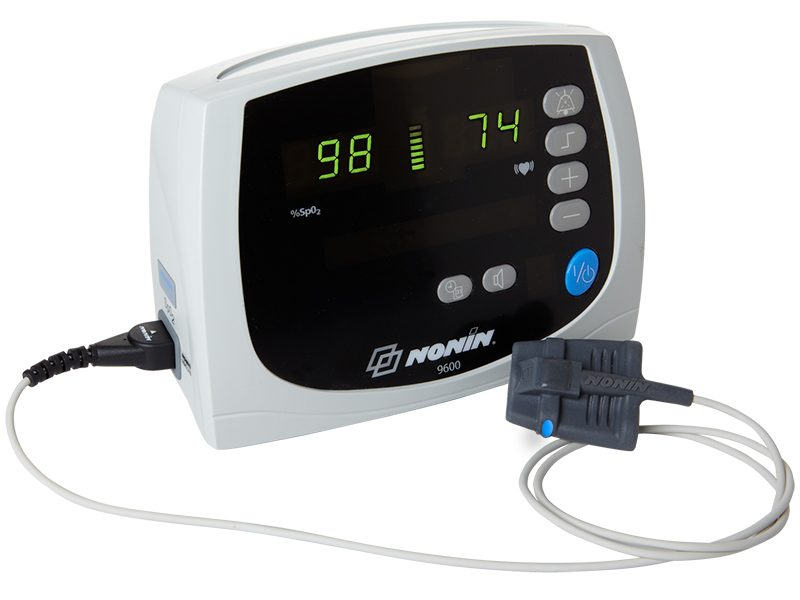
\includegraphics[width=.4\textwidth]{figures/validation/nonin_9600.jpg}
    \caption{The Nonin 9600 pulse oximeter used as validation in this project.}
    \label{fig:nonin_9600}
\end{figure}

\begin{figure}[t]
    \centering
    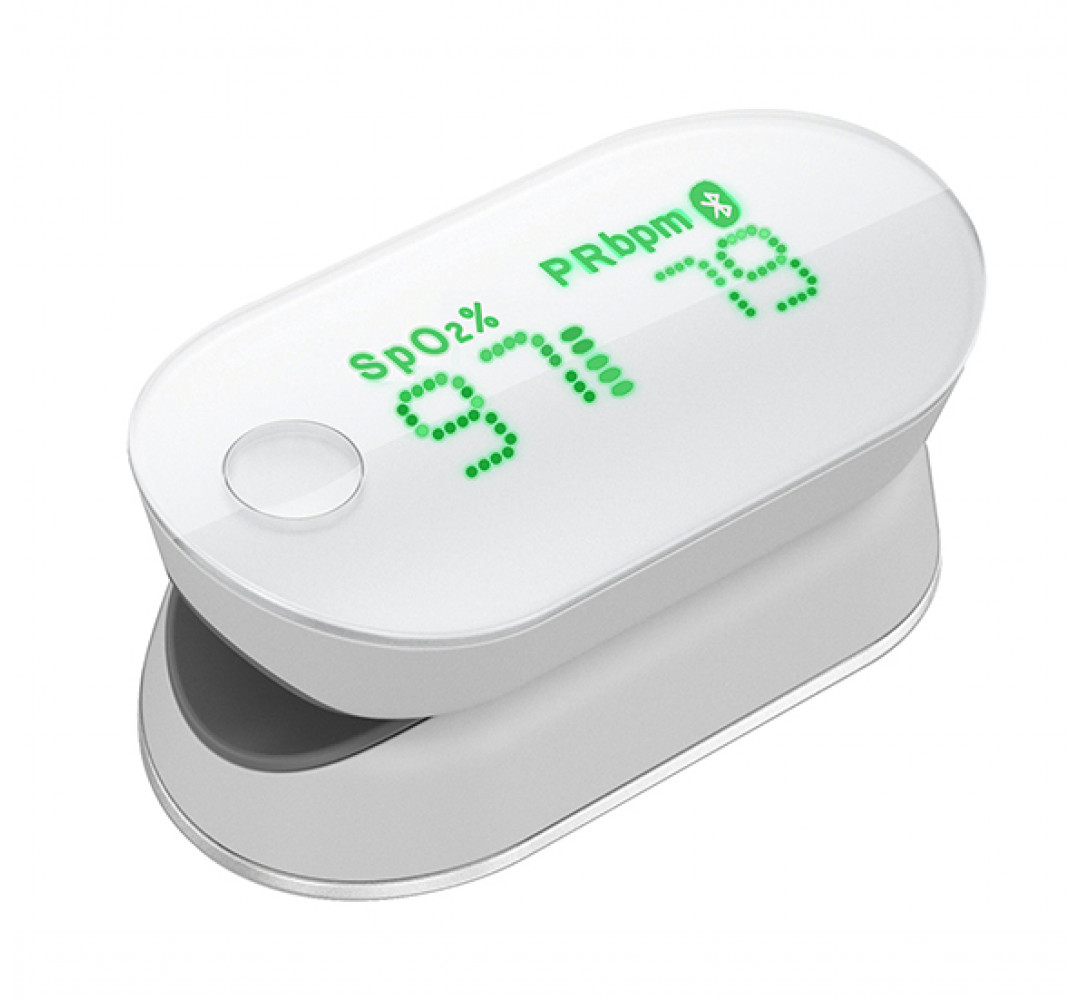
\includegraphics[width=.3\textwidth]{figures/validation/ihealth.jpg}
    \caption{The iHealth Air Pulse Oximeter used as validation in this project.}
    \label{fig:ihealth}
\end{figure}

\subsubsection{Respiratory rate validation}
While there are certainly devices which could measure respiration rate of a person, these devices were not present in the Erasmus MC, where the tests were performed. To still validate the respiration rate of a person, the following validation technique was developed. Since the person being measured is only sitting in front of the sensor and not doing any activities, the person is asked to count his own breaths. Every breath in and out counts as one breath, and each minute, this value is recorded and the counting starts again. This value counts as the validation for the respiration rate outputted by the IWR6843. This method has its downsides, people could forget to count, they could make a counting mistake, or they could start breathing non-naturally, since they are focusing on their breath. This is still the best way to measure the respiration rate during the project, but these downsides must be kept in mind when analyzing the validation results.

\subsection{External variables}
Variables outside of the sensor could also have an effect on the quality of the measurements. These variables contain among others the position in front of the sensor, the amount of people in front of the sensor and movement in the room.

\subsubsection{Position with respect to the sensor}
The IWR6843 is set up to measure persons within 0.3 to 2.5 meter range of the sensor, in the whole azimuth range, see also Figure~\ref{fig:range_metric}. The position of the person in the field of view of the sensor could play a role in the accuracy of the measurements.

\begin{figure}[t]
    \centering
    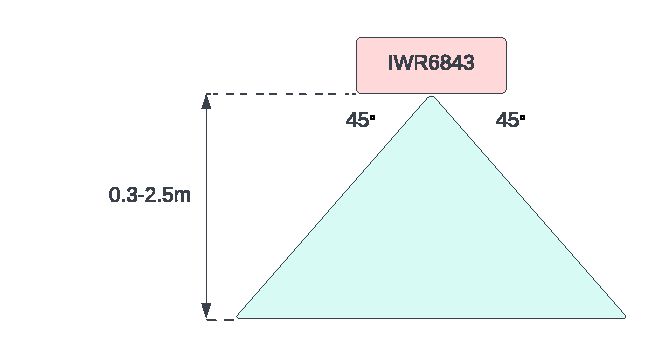
\includegraphics[width=.6\textwidth]{figures/validation/range_metric.pdf}
    \caption{Range and azimuth constraints of the sensor.}
    \label{fig:range_metric}
\end{figure}

\subsubsection{Amount of persons in front of the sensor}
The amount of persons that need to be measured is also a variable. It is possible that measurements of multiple persons close to each other will interfere.

\subsubsection{Background noise}
The sensor is very sensitive to noise. For the best result, the person needs to sit very still, and there needs to be as less noise as possible in the field of view of the sensor, to get a better SNR ratio.

\subsubsection{Height of the sensor}
The height of the sensor with respect to the chest region of the measured persons is very important. The sensor needs to be at the same height as the middle of the chest of the measured persons. Otherwise, the vibrations of the chest can't be picked up by the sensor and the measurements become unreliable.

\subsection{Person variables}
\label{sec:person_metrics}
The persons for which the vital signs are measured, all have different attributes. The most important ones are:

\begin{itemize}
    \item \textbf{sex:} there exist physical differences between men and women, also in the chest region where this project is focusing on. This metric could determine if men and woman are easier or more difficult to measure.
    \item \textbf{age:} the age of a person could contribute to multiple factors. A child is small, has a small chest region and could have a faster beating heart. Older persons are more likely to have extra body fat to dampen the vibrations produced by the heart and lungs.
    \item \textbf{weight/BMI:} body mass could have a big impact on the measurements. Positively, persons with a bigger weight are more likely to have a bigger chest region, so are easier to measure. Negatively, persons with more body mass are more likely to have extra fat on top of the chest, which could dampen the vibrations caused by the heart and lungs.
\end{itemize}

\section{Testing setup}
\label{sec:test_setup}
The testing environment is kept as consistent as possible. All of the equipment is placed on a desk, and in front of the desk one or more chairs are placed. The IWR6843ISK is set on the desk, with the antennae pointing to the chairs. Next to the IWR6843ISK the two Nonin 9600 pulse oximeters are placed, since the sensor leads are not that long. The IWR6843ISK and the two SpO2 sensors are connected to the computer via serial buses. The computer is operated by the operator. See also Figure~\ref{fig:test_setup} and Figure~\ref{fig:test_setup_pic}.

All tests have a duration of 5 minutes, or 300 seconds. The amount of 300 seconds has been chosen for multiple reasons. It gives the sensor time to stabilize. Because multiple buffers are used inside of the sensor, it takes some time before the buffers are filled with valid measurement data. Because the test subjects have walked to the testing location, it also gives the heart rate of the test subjects some time to settle in the heart rate during rest, which is the most stable.

\begin{figure}[t]
\begin{subfigure}{.45\textwidth}
  \centering
  % include first image
  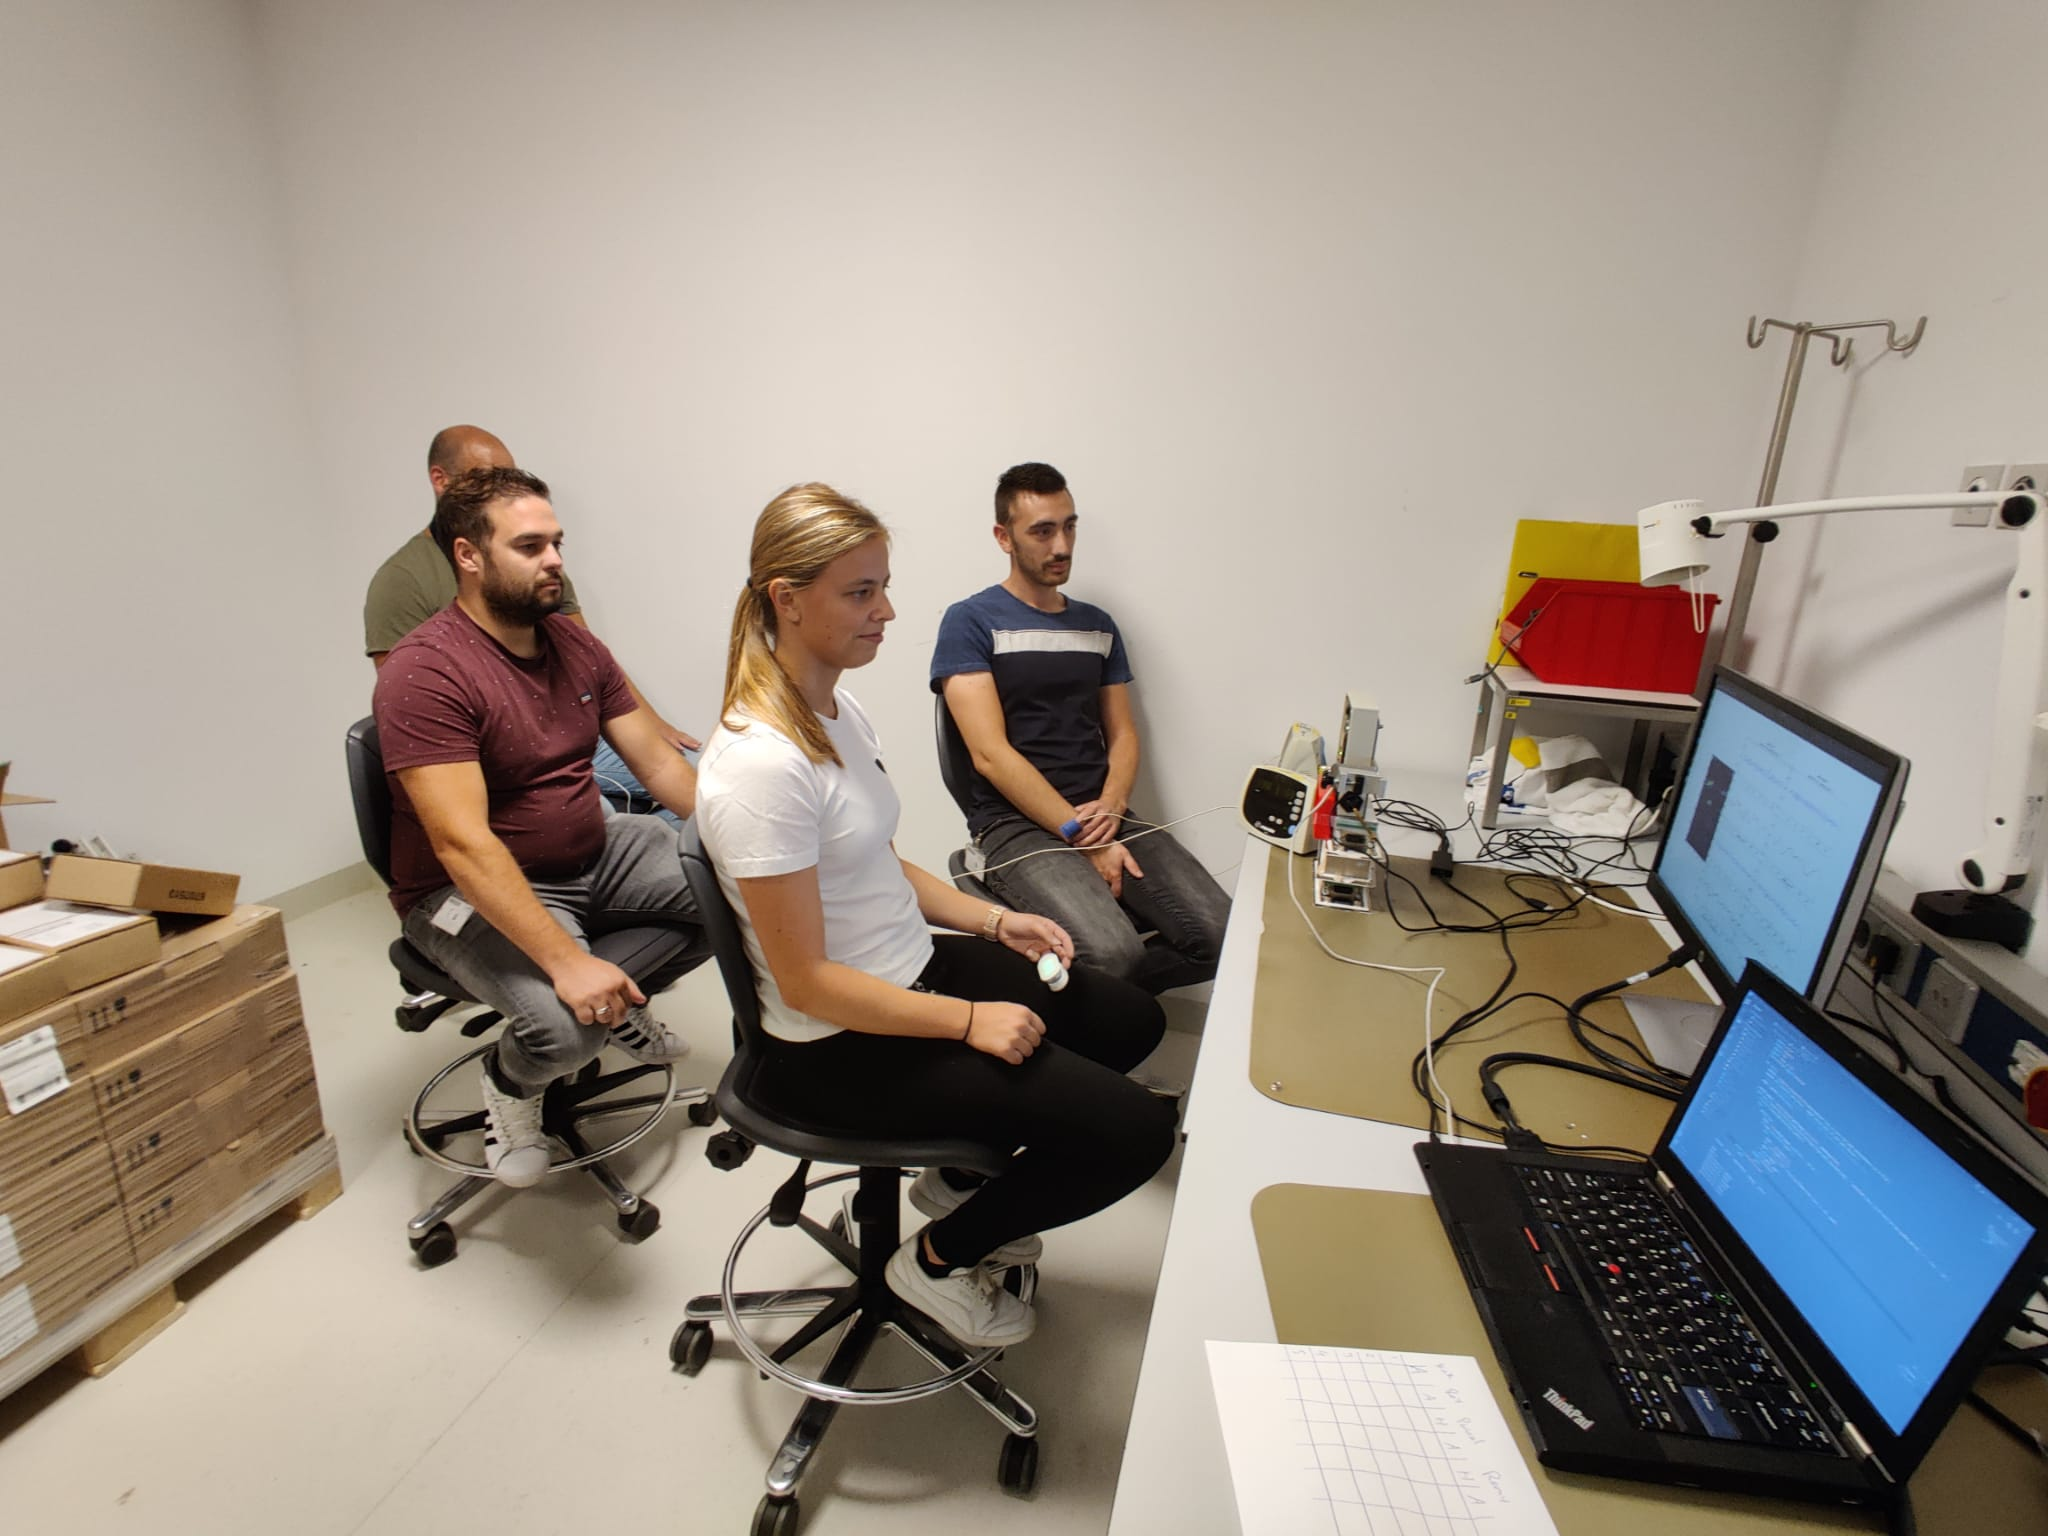
\includegraphics[width=\linewidth]{figures/validation/layout_4pers.jpeg}  
  \caption{Picture taken during the 4 persons vital sign estimation test.}
  \label{fig:test_setup_4_pic}
\end{subfigure}
\begin{subfigure}{.45\textwidth}
  \centering
  % include second image
  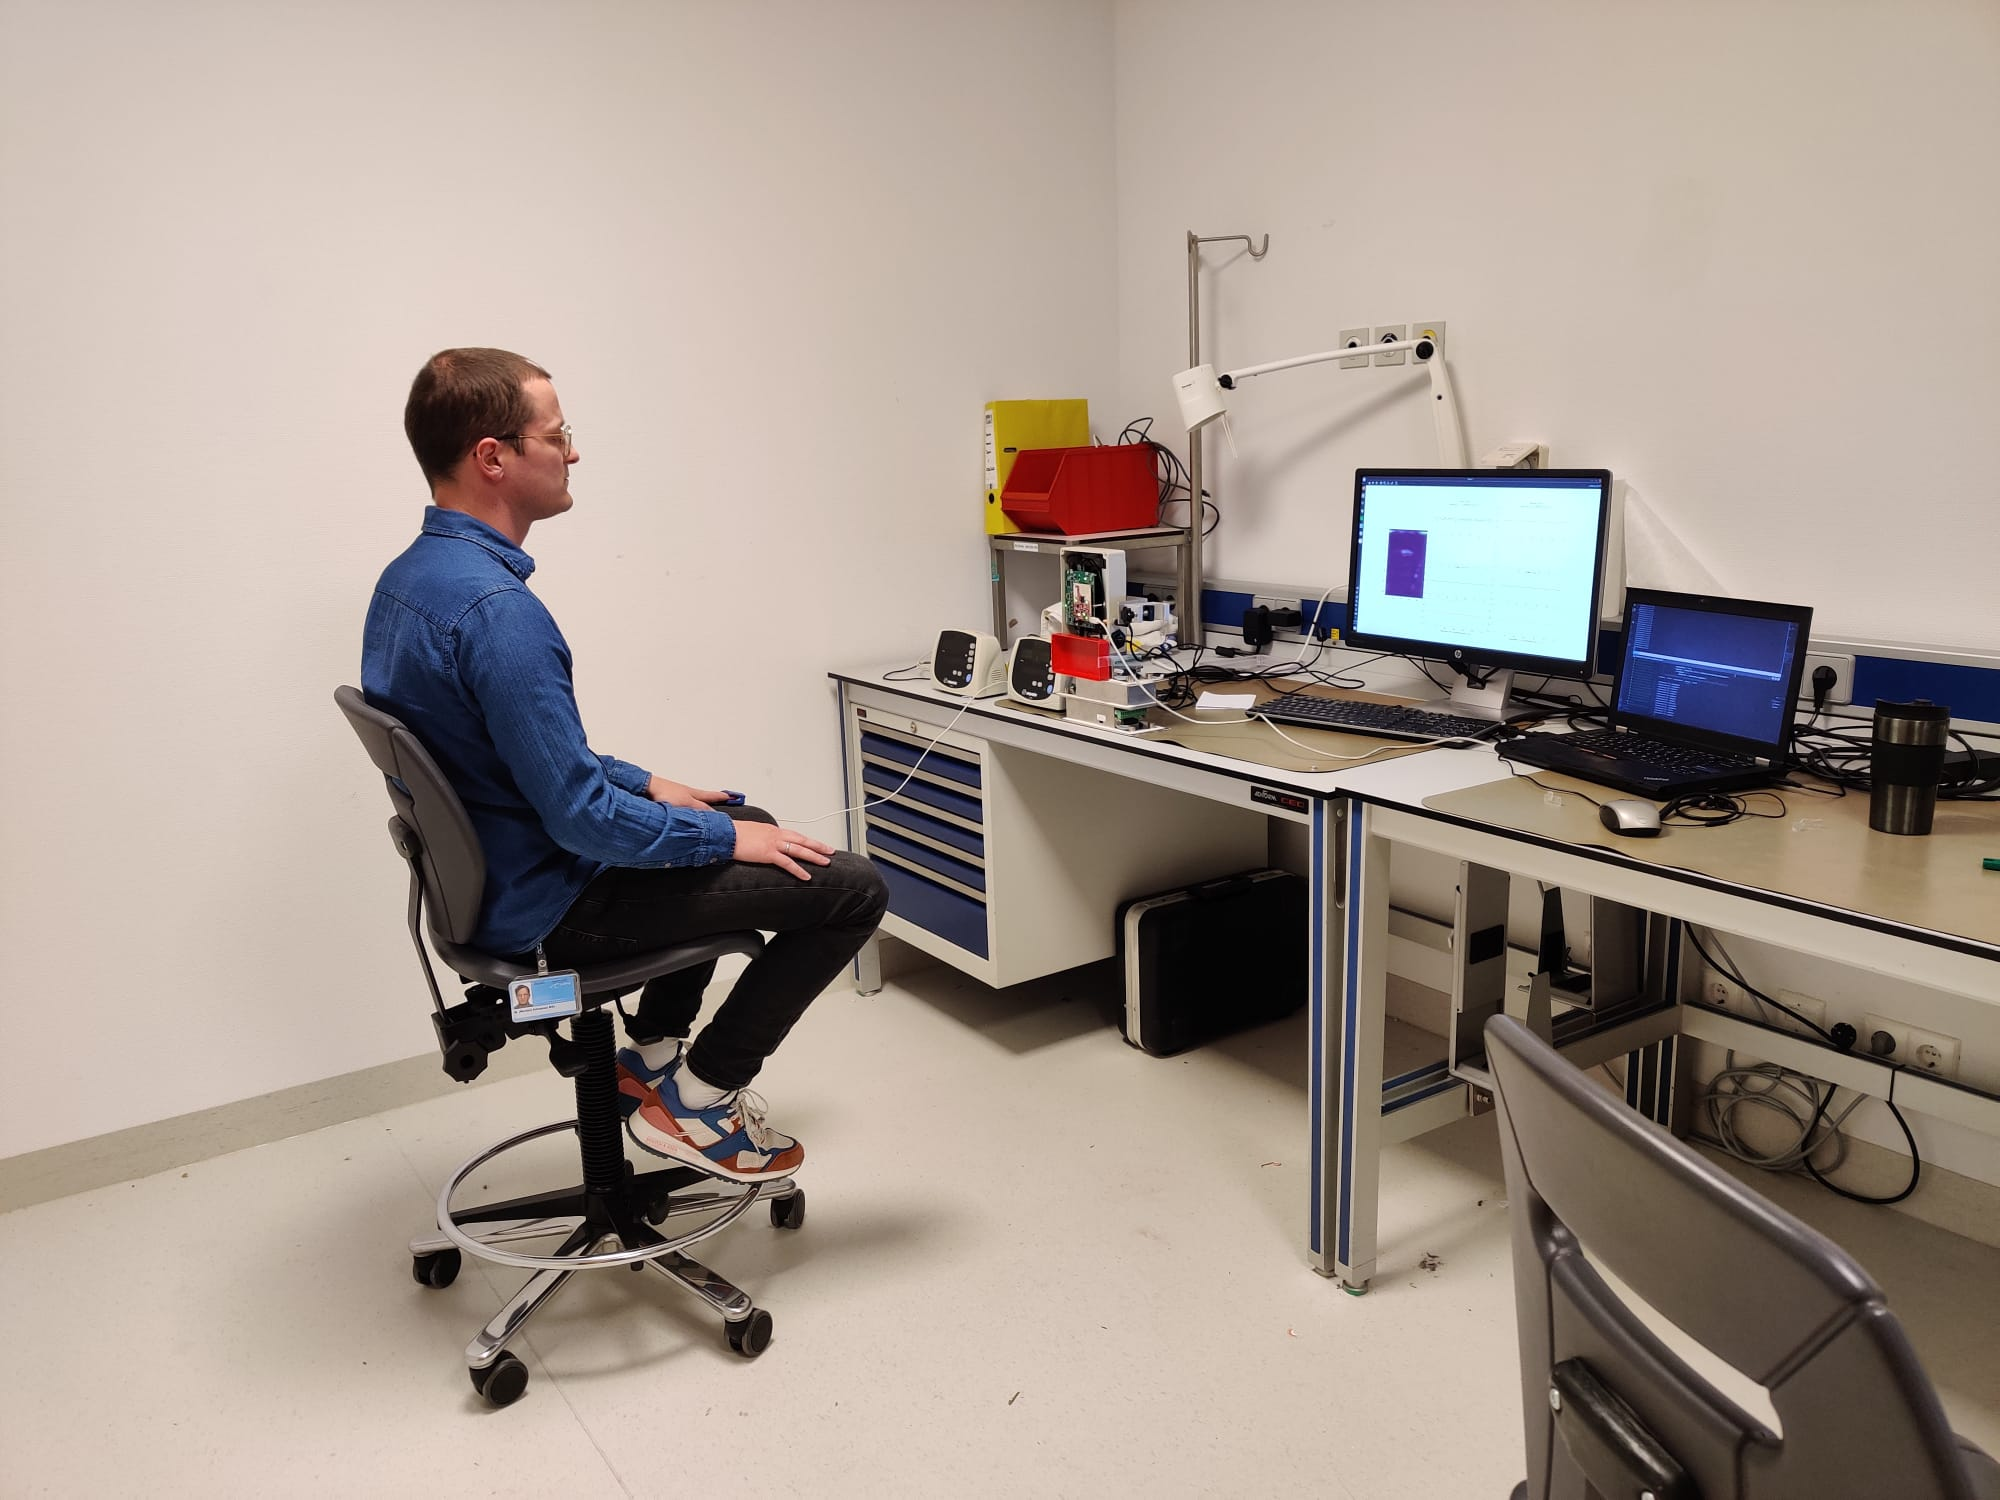
\includegraphics[width=\linewidth]{figures/validation/layout_michiel.jpeg}  
  \caption{Picture taken during the 1 person vital sign estimation test.}
  \label{fig:test_setup_1_pic}
\end{subfigure}
\caption{Two different tests being executed.}
\label{fig:test_setup_pic}
\end{figure}

\begin{figure}[t]
\begin{subfigure}{\textwidth}
  \centering
  % include first image
  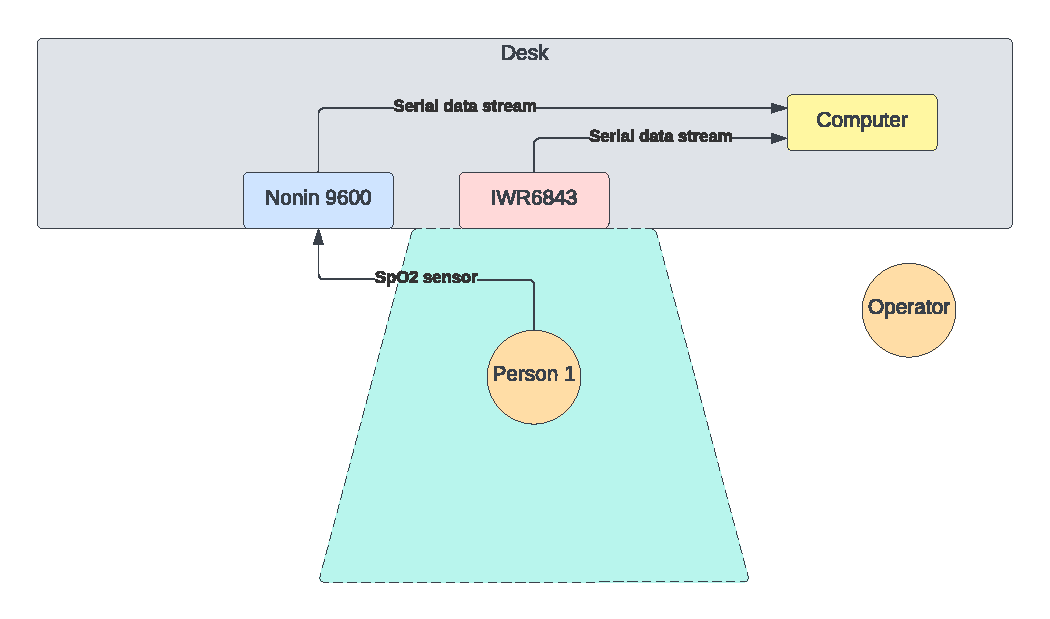
\includegraphics[width=.6\linewidth]{figures/validation/test_setup_1.pdf}  
  \caption{Test setup for vital sign estimation of 1 person.}
  \label{fig:test_setup_1}
\end{subfigure}
\begin{subfigure}{\textwidth}
  \centering
  % include second image
  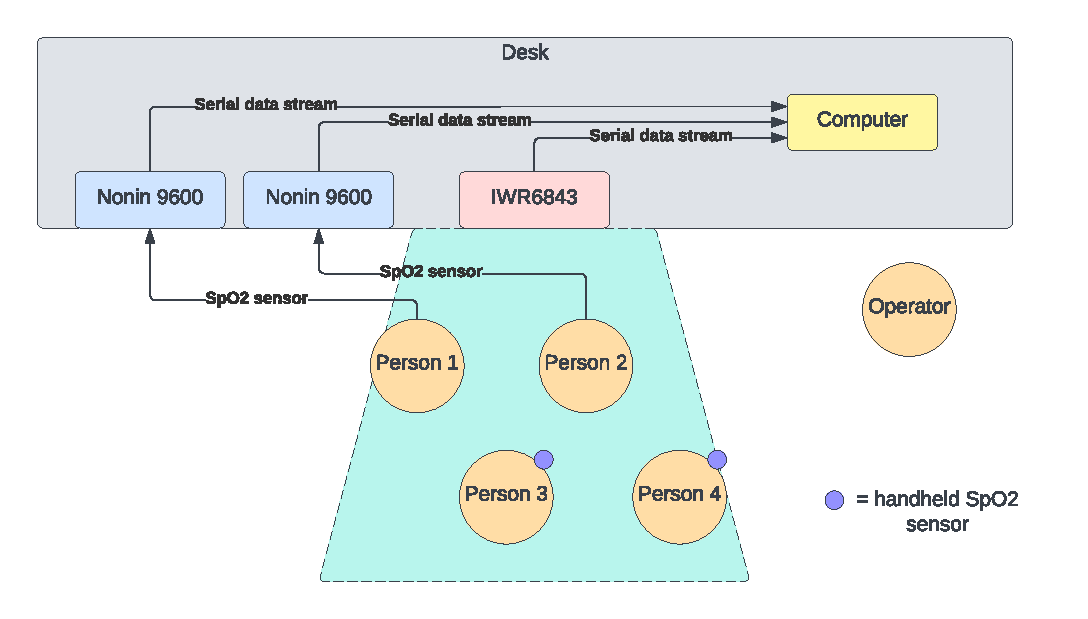
\includegraphics[width=.6\linewidth]{figures/validation/test_setup_4.pdf}  
  \caption{Test setup for the vital sign estimation of 4 persons.}
  \label{fig:test_setup_4}
\end{subfigure}
\caption{Two test setups being used to validate the project.}
\label{fig:test_setup}
\end{figure}

\section{Test subjects}
To properly validate the sensor, it has to be tested on persons. These test subjects were selected to reflect the validation plan. The test subjects are recorded for 5 minutes in a row, and along with the measurement data, additional metadata of the test subjects were recorded, as described in Section~\ref{sec:person_metrics}. This data includes age, gender, weight, length and additional comments. Using the weight and length, the BMI can be calculated. This data can be found in Table~\ref{tab:persons-info}.

Because the data which is being recorded is highly sensitive medical data, the names of the persons are anonymized. All of the persons also have signed an informed consent. These consent forms are stored in the archives of the 4TU Centre of Research Data, along with the measurement data itself in an encrypted form. 
% \todo{Add the informed consent forms to the appendix.}. 

\begin{table}[ht!]
\centering
\begin{tabular}{|l|l|l|l|l|l|l|}
\hline
Name & Age & Gender & \begin{tabular}[c]{@{}l@{}}Weight \\ (kg)\end{tabular} & \begin{tabular}[c]{@{}l@{}}Length \\ (m)\end{tabular} & BMI & Comments \\ \hline
P1 & 23 & male & 72 & 1.75 & 23 &  \\
P2 & 61 & female & 78 & 1.60 & 30 &  \\
P3 & 32 & male & 75 & 1.85 & 21 &  \\
P4 & 25 & male & 80 & 1.80 & 24 & \begin{tabular}[c]{@{}l@{}}Wore big layers \\ of clothing\end{tabular} \\
P5 & 26 & male & 100 & 1.80 & 30 & \begin{tabular}[c]{@{}l@{}}P5 was not detected \\ very well by the sensor\end{tabular} \\
P6 & 27 & male & 70 & 1.75 & 22 &  \\
P7 & 23 & male & 90 & 1.82 & 27 & \begin{tabular}[c]{@{}l@{}}Was a bit restless during \\ testing\end{tabular} \\
P8 & 43 & male & 80 & 1.82 & 24 &  \\
P9 & 49 & male & 85 & 1.85 & 24 &  \\
P10 & 35 & male & 86 & 1.77 & 27 &  \\
P11 & 49 & male & 92 & 1.80 & 28 &  \\
P12 & 23 & female & 62 & 1.75 & 20 &  \\
P13 & 76 & male & 91 & 1.75 & 29 &  \\
P14 & 75 & female & 82 & 1.65 & 30 &  \\
P15 & 46 & female & 58 & 1.7 & 20 &  \\
P16 & 23 & male & 68 & 1.76 & 21 &  \\\hline
\end{tabular}
\caption{All of the recorded metadata from the test subjects.}
\label{tab:persons-info}
\end{table}

\section{Results}
\subsection{One person validation}
\label{sec:one_pers_validation}
The validation of the vital signs of one person in front of the sensor is an important part of the validation process. Because the vital sign estimation of one person is the same process as the vital sign estimation of multiple persons, the validation of one person was used to partially validate multiple person vital signs. To validate the general accuracy of the project, 12 persons have been tested, all individually. The test setup can be found in Section~\ref{sec:test_setup}. 

For each recorded heart rate and respiration rate from the IWR6843, it is compared against the control heart rate and respiration rate. For each test subject, the average accuracy percentage is calculated. The accuracy percentage is how much the measurement from the IWR6843 differs from the control measurement. The percentage is calculated using the formula in Eq.~\ref{eq:deviation_calculation}.

\begin{equation}
    accuracy = abs(M_{IWR6843} - M_{control}) / M_{control}
    \label{eq:deviation_calculation}
\end{equation}

These averaged percentages can be found in Table~\ref{tab:one-person-results}. The most accurate measurement and the least accurate measurement are drawn in this thesis. For the most accurate result, see Figure~\ref{fig:roy_meas}. For the least accurate result, see Figure~\ref{fig:tim_meas}.
% \todo{Incorporate averages from the whole measurement?}
% \todo{Replace with P13?}

In later sections, more details are provided of the relation between personal variables and the detected accuracy of the measurements. For now, only observations are done on individual measurements. The first observation is the difference in deviation between Table~\ref{tab:one-person-results} and Table~\ref{tab:one-person-results_2}. This is because the percentage in Table~\ref{tab:one-person-results} is calculated for each measurement. For 300 seconds of recording, 1200 measurements are gathered. These 1200 percentages get averaged into one percentage. For Table~\ref{tab:one-person-results_2}, the measurements from the control and from the IWR6843 are first averaged, and then the deviation percentage is calculated. Because the measurements from the IWR6843 are quite noisy, the deviation percentages in Table~\ref{tab:one-person-results} are higher than Table~\ref{tab:one-person-results_2}.

Another way to visualize the data is to generate a Bland-Altman plot. This plot is specifically designed to plot out the agreement of two different measurement devices. In the case of this project, that would be the radar measurement and the control measurement. In this graph, the mean difference and the standard deviation between the two measurement types are being given. The Bland-Altman plot for the heart rate comparison of all one person validation tests can be found in Figure~\ref{fig:ba_one_heart}. The Bland-Altman plot for the respiration rate can be found in Figure~\ref{fig:ba_one_breath}.

\begin{figure}[t]
    \centering
    \hspace*{-2cm}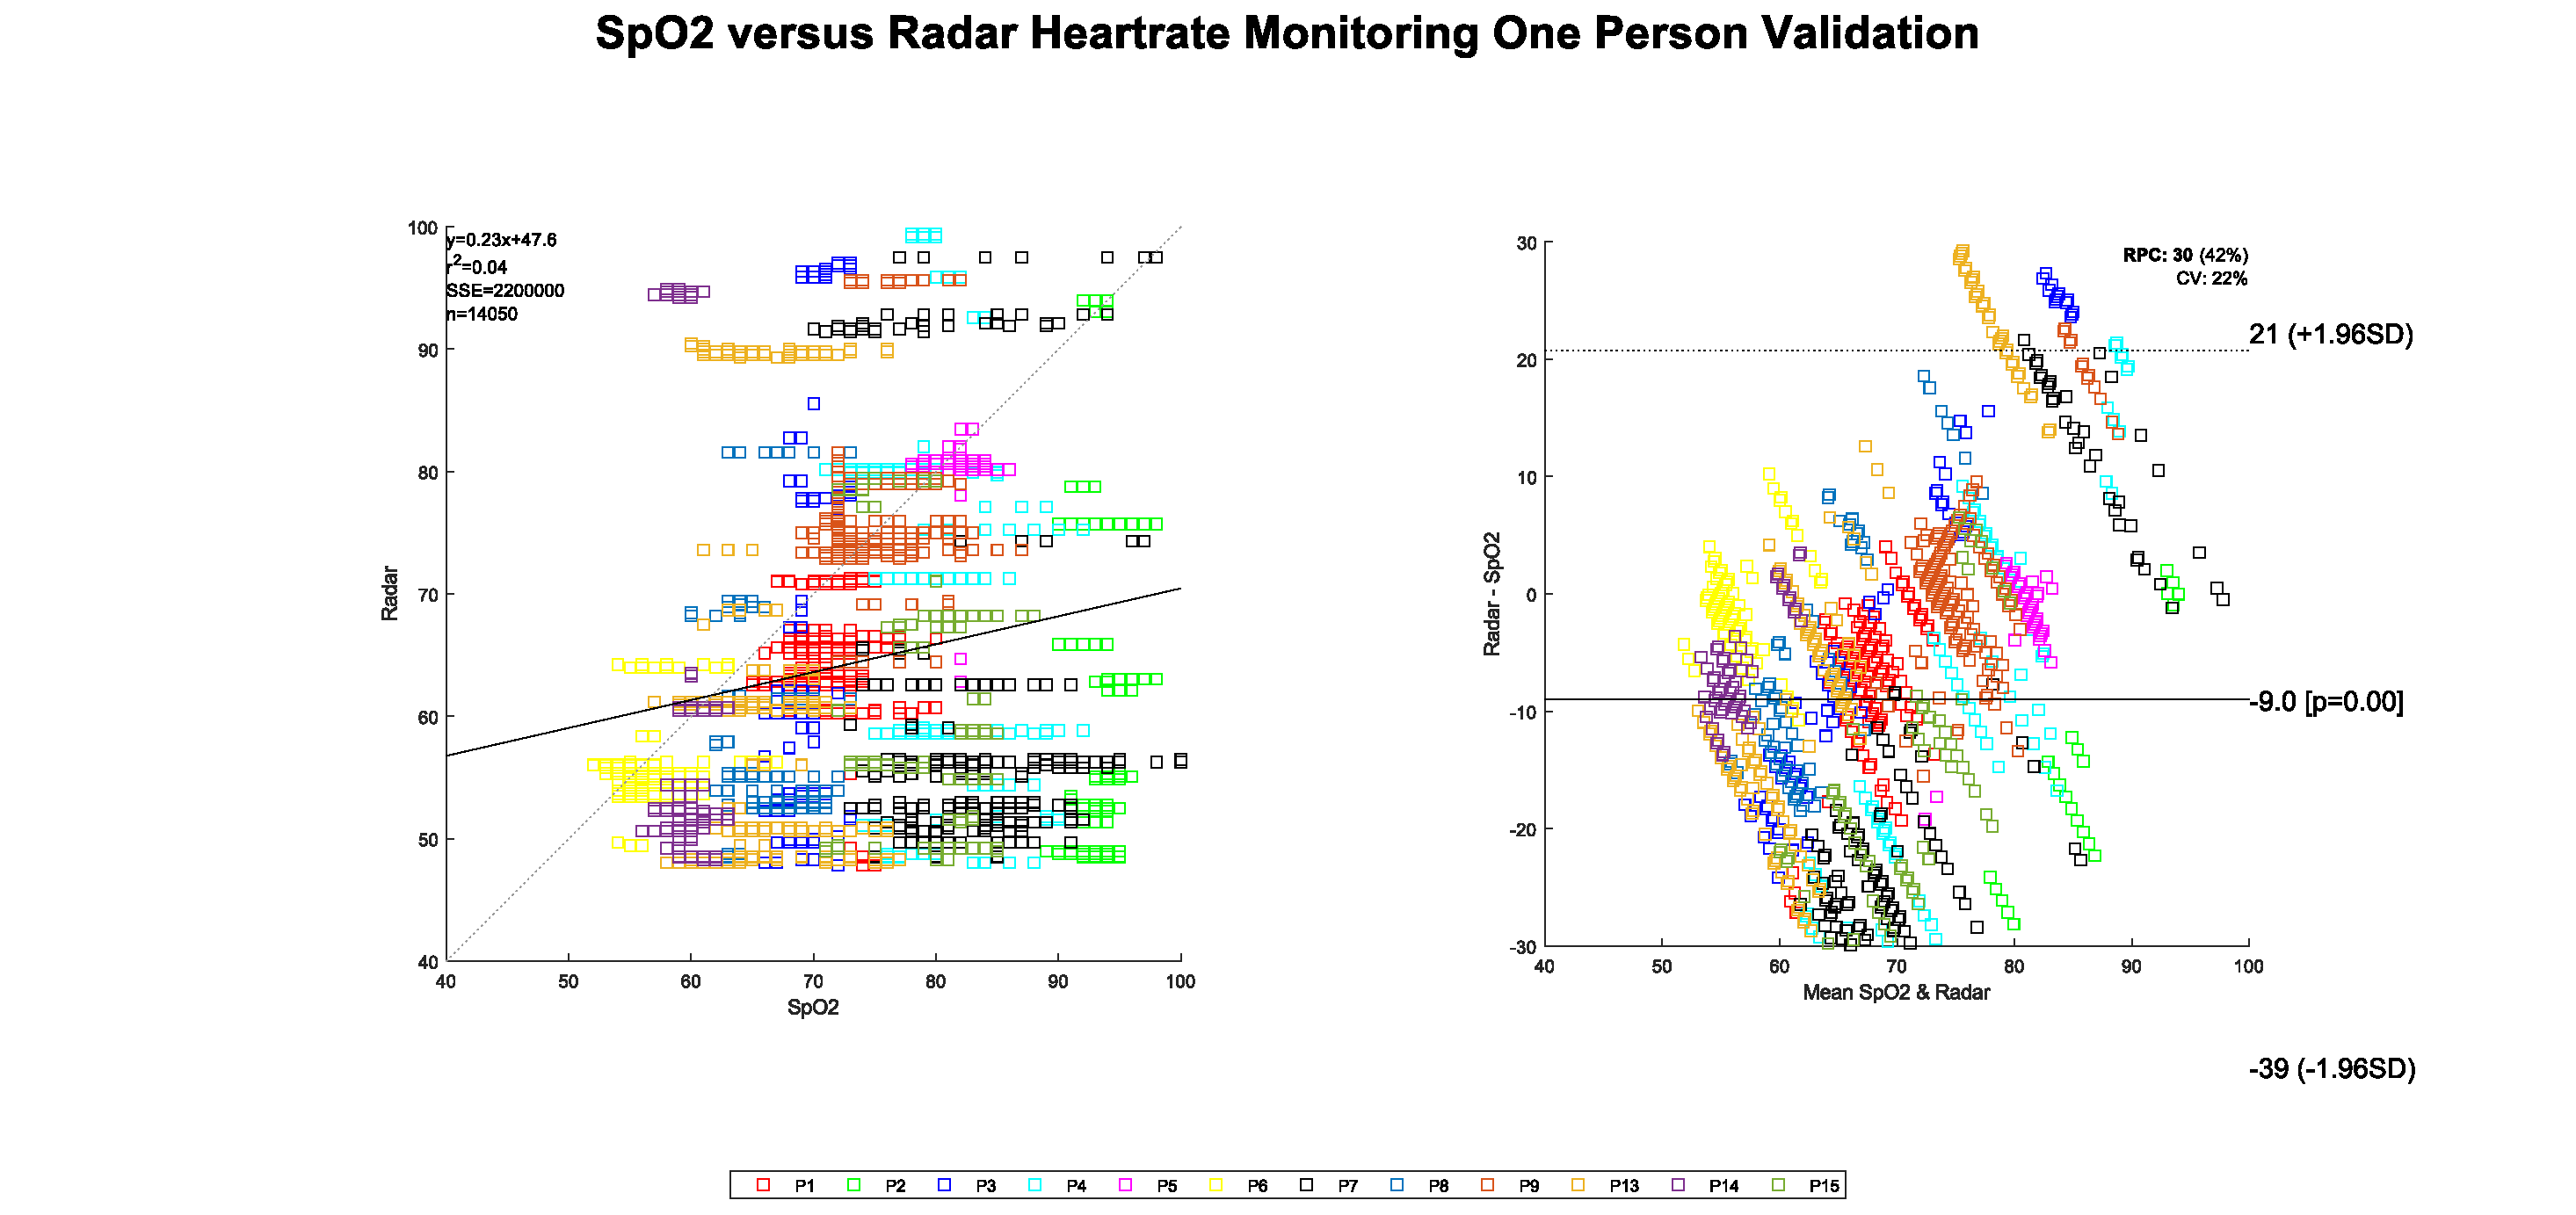
\includegraphics[width=1.2\textwidth]{figures/validation/bland_altman2.pdf}
    \caption{Bland-Altman plot of all one person heart rate validation results.}
    \label{fig:ba_one_heart}
\end{figure}

\begin{figure}[t]
    \centering
    \hspace*{-2cm}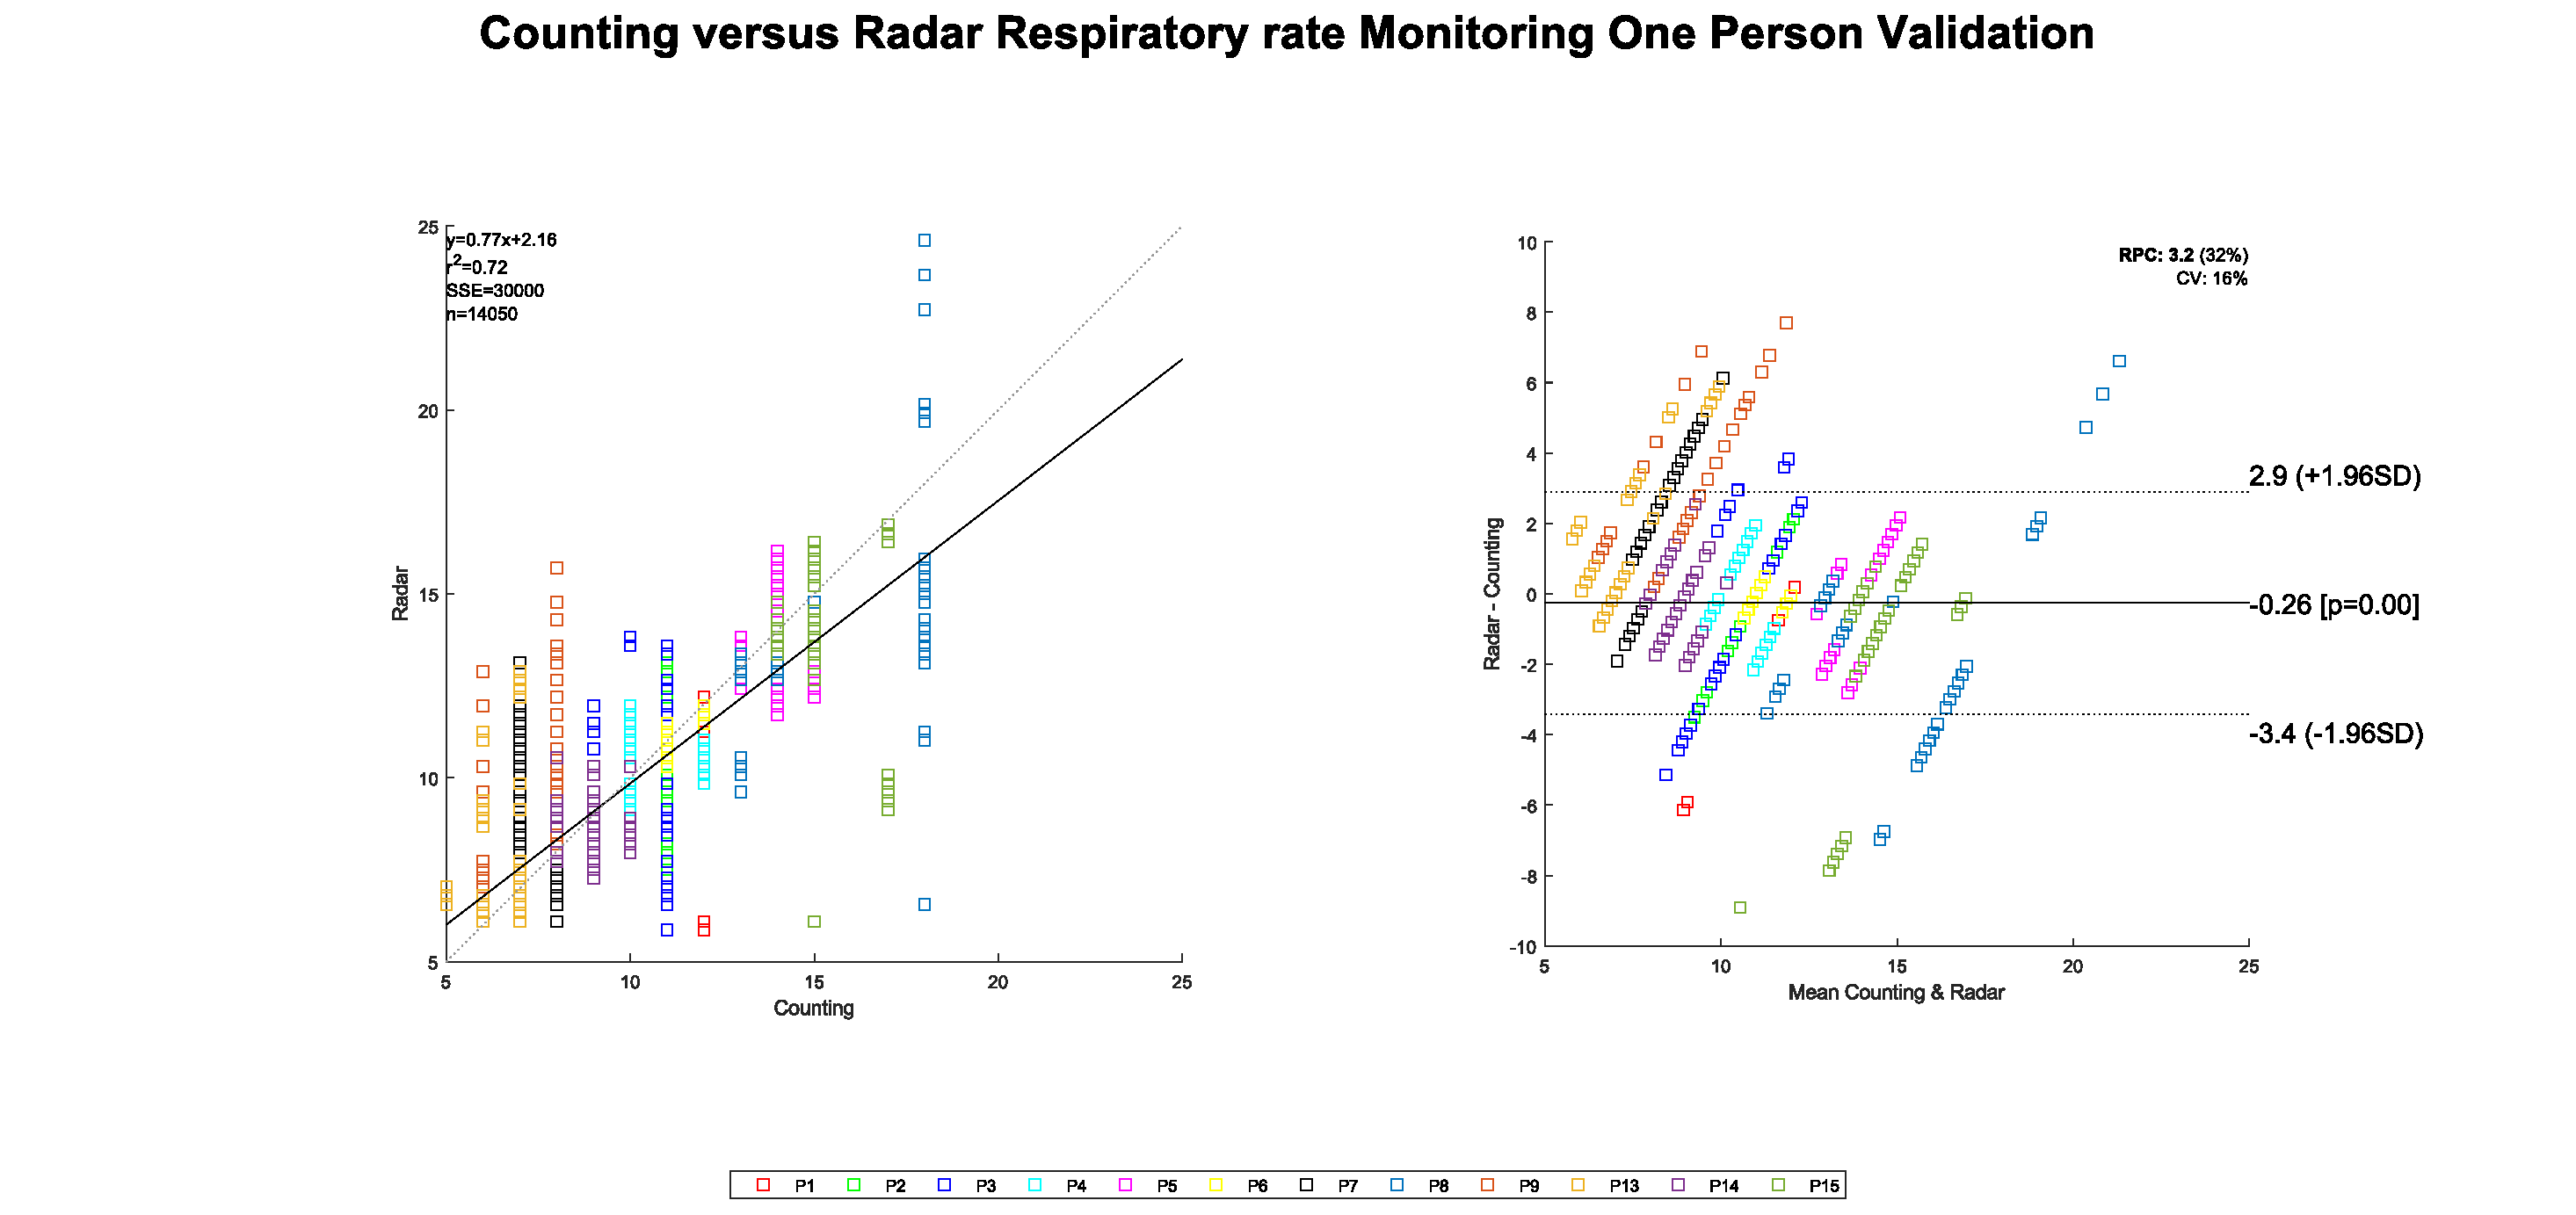
\includegraphics[width=1.2\textwidth]{figures/validation/bland_altman_BR.pdf}
    \caption{Bland-Altman plot of all one person respiratory rate validation results.}
    \label{fig:ba_one_breath}
\end{figure}

The average heart rate estimation accuracy of the sensor is 10.86\%. This is mainly due to four persons where the measurement accuracy was worse compared to the other 7 measured persons. For three of the four persons a reason can be found for this lesser accuracy, see also the remarks in Table~\ref{tab:persons-info}. \emph{P4} had multiple layers of thick clothing on, which could distort the signal. \emph{P5} was not detected by the people detection algorithm very well, so the quality of the data to do the vital signs estimation on was not very high. \emph{P9} has lung problems, which express in a higher and more unstable respiration rate and heart rate. For the lower accuracy of \emph{P13} there is no clear explanation, except an higher BMI, which will be discussed in Section~\ref{sec:weight_res}. Taking out these four lower accuracy's, the average accuracy drops down to 3.30\%.

The respiration accuracy averaged around all the persons tested is 7.61\%. But, when looking at the breathing rate numbers in Table~\ref{tab:one-person-results_2}, the difference between the control- and the sensor measurement is either 0 or 1. Only at \emph{P5} there exists a difference in measurements of 2, but this could again be due to the people detection algorithm not detecting the person properly. Since the control measurements are counted by the persons themselves, part of this accuracy number could be due to miscounting.

To conclude, the one person vital signs estimation works. Especially the respiration rate is exactly right or only one off. The heart rate estimation accuracy is around 10\%. The reason for this lower accuracy could be that the heart rate is faster than the respiration rate and the magnitude of the vibrations is smaller. This accuracy could be improved by tweaking the algorithms and the algorithm parameters.

\begin{table}[ht]
\centering
\begin{tabular}{|r|c|c|l|}
\hline
Person & \begin{tabular}[c]{@{}c@{}}Heart rate \\ accuracy\end{tabular} & \begin{tabular}[c]{@{}c@{}}Respiratory \\ rate accuracy\end{tabular} & \textbf{Average} \\ \hline
P1 & 91.8\% & 93.4\% & \textbf{92.6\%} \\
P2 & 98.3\% & 90.5\% & \textbf{94.4\%} \\
P3 & 95.3\% & 98.0\% & \textbf{96.7\%} \\
P4 & 70.3\% & 88.9\% & \textbf{79.6\%} \\
P5 & 83.3\% & 91.5\% & \textbf{87.4\%} \\
P6 & 94.5\% & 84.3\% & \textbf{89.4\%} \\
P7 & 79.4\% & 76.1\% & \textbf{77.7\%} \\
P8 & 83.2\% & 86.5\% & \textbf{84.8\%} \\
P9 & 75.2\% & 92.1\% & \textbf{83.7\%} \\
P13 & 64.6\% & 86.9\% & \textbf{75.7\%} \\
P14 & 81.2\% & 83.4\% & \textbf{82.3\%} \\ \hline
\textbf{Average} & \textbf{82.6\%} & \textbf{86.3\%} & \textbf{84.4\%} \\ \hline
\end{tabular}
\caption{One person vital signs estimation validation results. The percentage denotes the absolute difference between the IWR6843 heart- and respiration rate, and the control rates.}
\label{tab:one-person-results}
\end{table}

\begin{table}[ht]
\centering
\begin{tabular}{|r|c|c|l|c|c|l|}
\hline
\textbf{Person} & \textbf{\begin{tabular}[c]{@{}c@{}}Heart rate \\ SpO2 \\ sensor\end{tabular}} & \textbf{\begin{tabular}[c]{@{}c@{}}Heart rate\\ IWR6843\end{tabular}} & \textbf{\begin{tabular}[c]{@{}l@{}}Heart rate\\ accuracy\end{tabular}} & \textbf{\begin{tabular}[c]{@{}c@{}}Respi\\ ratory\\ rate\end{tabular}} & \textbf{\begin{tabular}[c]{@{}c@{}}Respi\\ ratory\\ rate \\ IWR6843\end{tabular}} & \textbf{\begin{tabular}[c]{@{}l@{}}Respi\\ ratory\\ rate \\ accuracy\end{tabular}} \\ \hline
\textbf{P1} & 71 & 65 & \textbf{92.0\%} & 10 & 9 & \textbf{93.3\%} \\
\textbf{P2} & 81 & 81 & \textbf{99.5\%} & 14 & 13 & \textbf{93.1\%} \\
\textbf{P3} & 56 & 56 & \textbf{98.7\%} & 11 & 11 & \textbf{99.5\%} \\
\textbf{P4} & 83 & 62 & \textbf{74.2\%} & 8 & 8 & \textbf{97.2\%} \\
\textbf{P5} & 66 & 59 & \textbf{89.2\%} & 15 & 13 & \textbf{91.7\%} \\
\textbf{P6} & 75 & 76 & \textbf{98.6\%} & 6 & 7 & \textbf{85.8\%} \\
\textbf{P7} & 66 & 63 & \textbf{96.4\%} & 6 & 7 & \textbf{80.8\%} \\
\textbf{P8} & 60 & 57 & \textbf{96.2\%} & 9 & 9 & \textbf{92.4\%} \\
\textbf{P9} & 80 & 60 & \textbf{75.52\%} & 15 & 15 & \textbf{95.4\%} \\
\textbf{P13} & 94 & 61 & \textbf{64.7\%} & 11 & 10 & \textbf{92.2\%} \\
\textbf{P14} & 69 & 66 & \textbf{95.5\%} & 10 & 10 & \textbf{95.0\%} \\ \hline
\textbf{Average} & \textbf{} & \textbf{} & \textbf{89.1\%} &  &  & \textbf{92.4\%} \\ \hline
\end{tabular}
\caption{One person vital signs estimation validation results. The average heart rates and respiratory rates of all sensors from the whole reading, with the absolute deviation between the control measurements and the IWR6843 measurements.}
\label{tab:one-person-results_2}
\end{table}

\begin{figure}[t]
\begin{subfigure}{\textwidth}
  \centering
  % include first image
  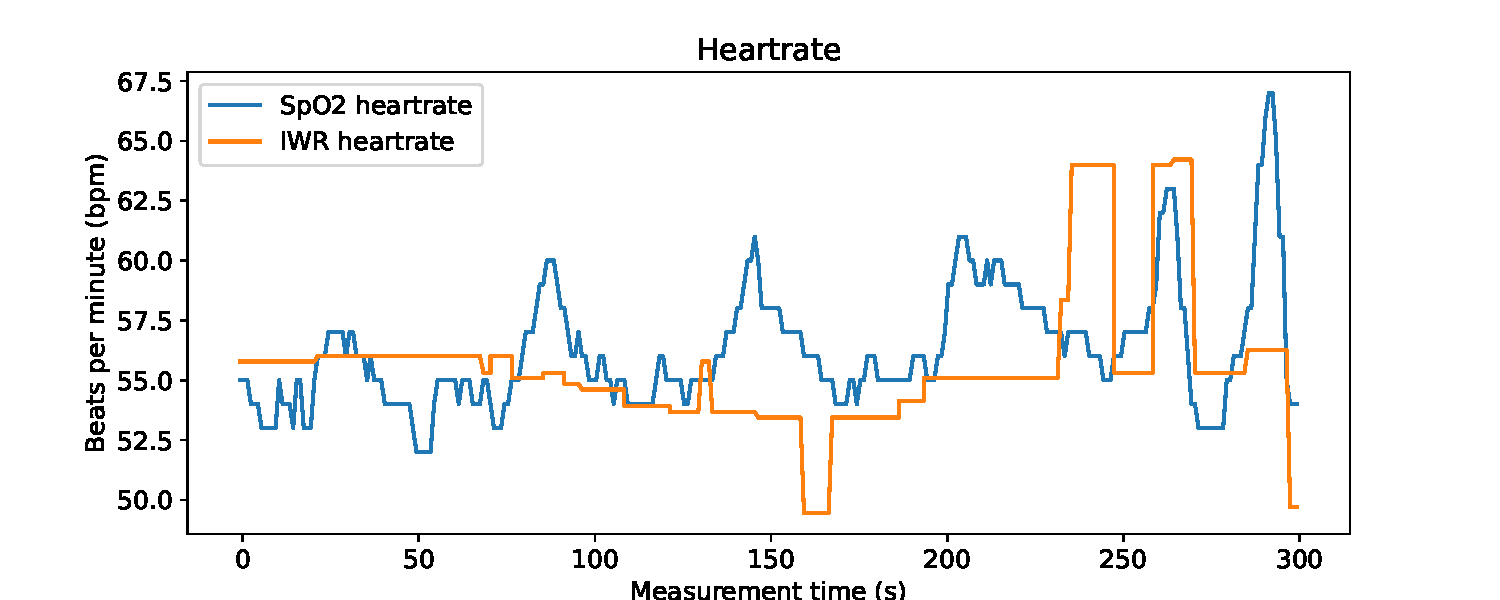
\includegraphics[width=\linewidth]{figures/validation/roy_heart.pdf}  
  \caption{The IWR6843 estimated heart rate and the SpO2 sensor heart rate from \emph{P3} plotted out.}
  \label{fig:roy_heart}
\end{subfigure}
\begin{subfigure}{\textwidth}
  \centering
  % include second image
  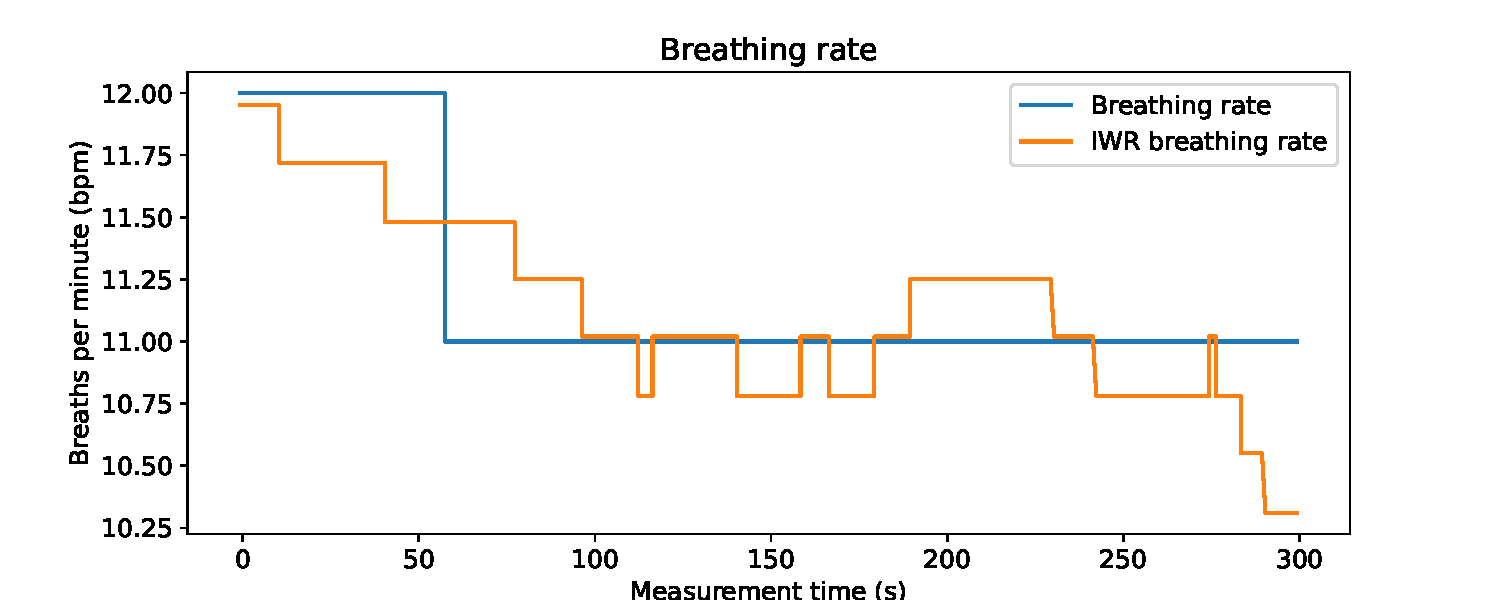
\includegraphics[width=\linewidth]{figures/validation/roy_breath.pdf}  
  \caption{The IWR6843 estimated respiratory rate and the counted respiratory rate from \emph{P3} plotted out.}
  \label{fig:roy_breath}
\end{subfigure}
\caption{Validation data from \emph{P3}. This is the most accurate result in the one person validation section.}
\label{fig:roy_meas}
\end{figure}

\begin{figure}[t]
\begin{subfigure}{\textwidth}
  \centering
  % include first image
  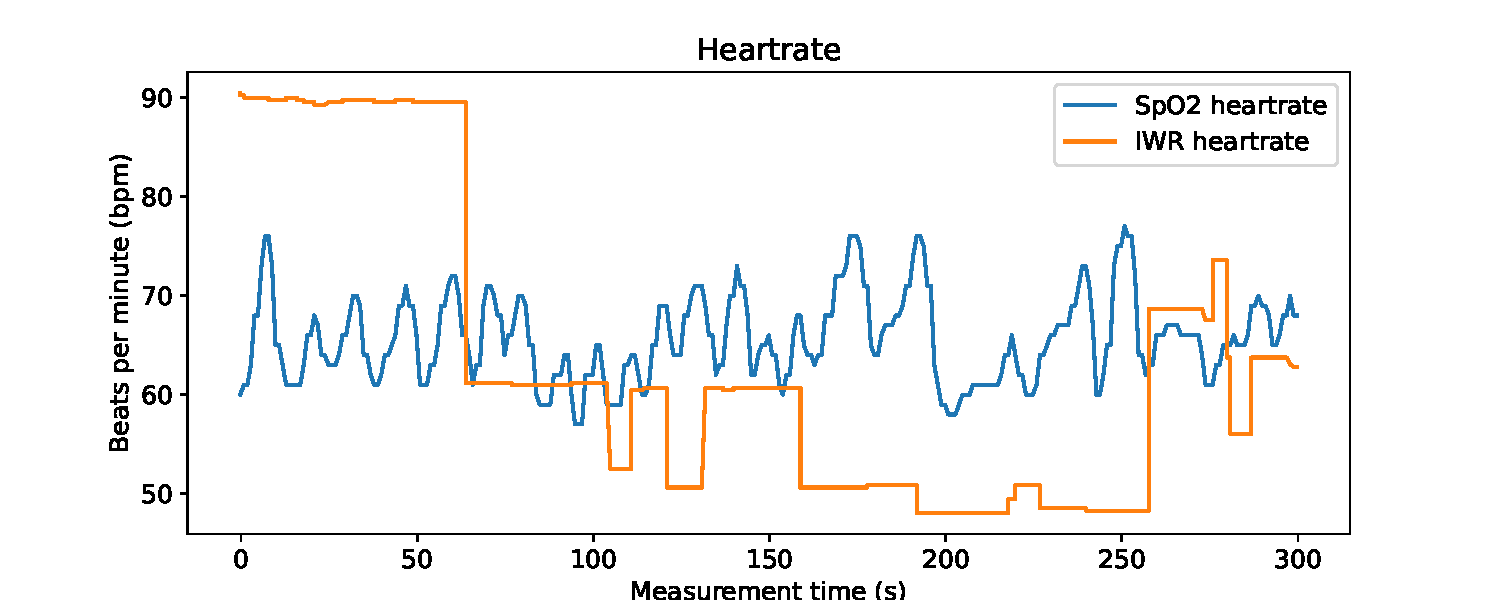
\includegraphics[width=\linewidth]{figures/validation/tim_heart.pdf}  
  \caption{The IWR6843 estimated heart rate and the SpO2 sensor heart rate from \emph{P7} plotted out.}
  \label{fig:tim_heart}
\end{subfigure}
\begin{subfigure}{\textwidth}
  \centering
  % include second image
  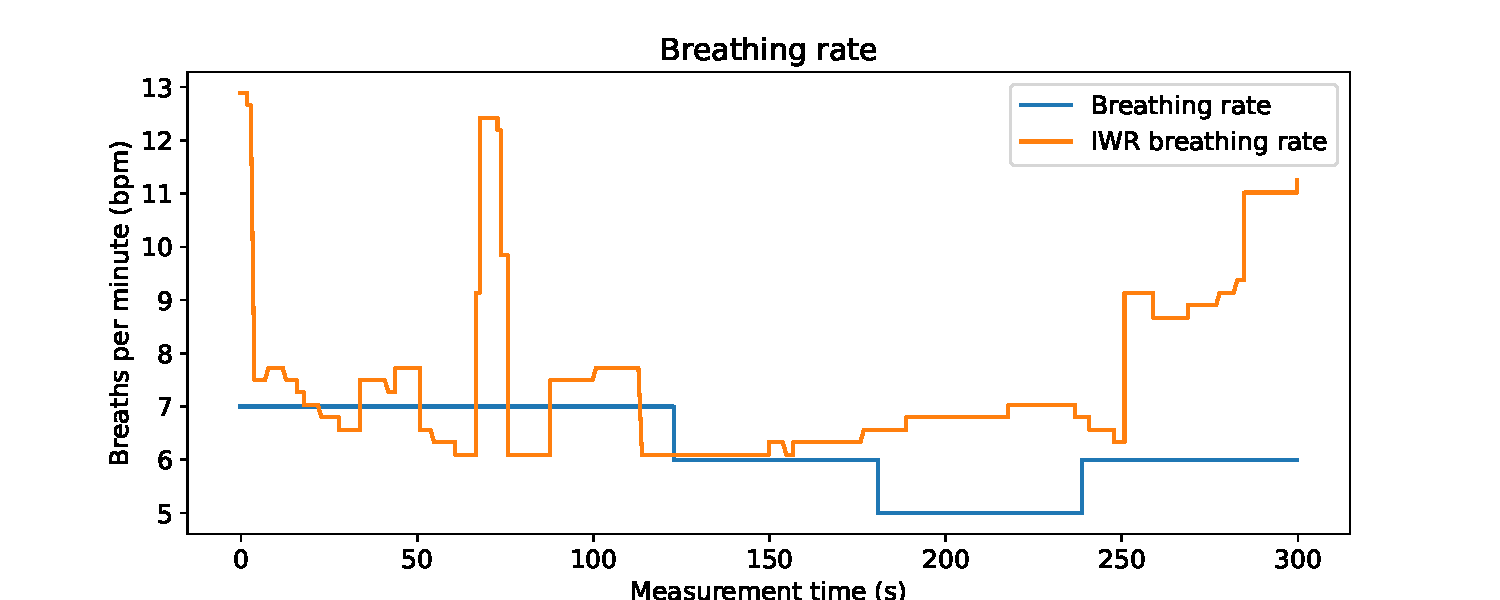
\includegraphics[width=\linewidth]{figures/validation/tim_breath.pdf}  
  \caption{The IWR6843 estimated respiratory rate and the counted respiratory rate from \emph{P7} plotted out.}
  \label{fig:tim_breath}
\end{subfigure}
\caption{Validation data from \emph{P7}. This is the least accurate result in the one person validation section.}
\label{fig:tim_meas}
\end{figure}

\subsection{Two person validation}
An important step for this project is moving on from measuring one test subject to two test subjects at the same time. The most important question to answer is if the measurement from one test subject can influence the measurement from another test subject. The test setup is the same as in Figure~\ref{fig:test_setup_4}, with the exception that only the first row is in use. The other deviation is that only one Novim 9600 was available to measure heart rate, so the other heart rate is measured using the iHealth device, see also Section~\ref{sec:heartrate_validation}.

The results from this validation can be found in Table~\ref{tab:two-person-results_2}. The first observation which immediately stands out is that the estimation for one test subject is almost perfect, while the estimation for the other test subject is far from perfect. In the next Section (\ref{sec:four-person-validation}), four test subjects are measured at the same time, and there the accuracy is higher. No explanation can be found for this large difference in accuracy.

\begin{table}[ht]
\centering
\begin{tabular}{|r|c|c|l|c|c|l|}
\hline
\textbf{Person} & \textbf{\begin{tabular}[c]{@{}c@{}}Heart rate \\ SpO2 \\ sensor\end{tabular}} & \textbf{\begin{tabular}[c]{@{}c@{}}Heart rate\\ IWR6843\end{tabular}} & \textbf{\begin{tabular}[c]{@{}l@{}}Heart rate\\ accuracy\end{tabular}} & \textbf{\begin{tabular}[c]{@{}c@{}}Respi\\ ratory\\ rate\end{tabular}} & \textbf{\begin{tabular}[c]{@{}c@{}}Respi\\ ratory\\ rate \\ IWR6843\end{tabular}} & \textbf{\begin{tabular}[c]{@{}l@{}}Respi\\ ratory\\ rate \\ accuracy\end{tabular}} \\ \hline
\textbf{P15} & 83 & 57 & \textbf{68.8\%} & 12 & 11 & \textbf{85.0\%} \\
\textbf{P16} & 71 & 69 & \textbf{97.2\%} & 10 & 10 & \textbf{91.7\%} \\ \hline
\textbf{Average} & \textbf{} & \textbf{} & \textbf{83.0\%} &  &  & \textbf{88.3\%} \\ \hline
\end{tabular}
\caption{Two person vital signs estimation validation results. The average heart rates and respiratory rates of all sensors from the whole reading, with the absolute deviation between the control measurements and the IWR6843 measurements.}
\label{tab:two-person-results_2}
\end{table}

\subsection{Four person validation}
\label{sec:four-person-validation}
% - How the validation was done
% - The results
% - difficulty with the people detection
% - less accurate results
For this project, estimating the vital signs of 4 persons at the same time is the maximum. There are two reasons for this number. Firstly, because of the resource-heavy algorithms this is all the chip can handle at the moment because of timing constraints. Secondly, because the measurements take place in the range of 0.3 to 2.5 meters from the sensor, it becomes too crowded in front of the sensor with more than 4 persons. 

To validate the accuracy of measuring four vital signs at the same time, four persons were put in front of the sensor, as can be observed in Figure~\ref{fig:test_setup_4} and Figure~\ref{fig:test_setup_4_pic}. The rest of the validation procedure stays the same, the test is run for 5 minutes with the persons sitting statically. All of the chests of the four persons are at the same height of the sensor antennae. 

The most uncertain part of this validation was if the person detection would work reliably. Not only one, but four persons must be detected and remain detected during the 5 minutes of testing time. Luckily, the person detection remained stable during the test, and apart from a few glitches the four persons remained detected during the test, see also Figure~\ref{fig:4_persons_detected}.

\begin{figure}[t]
    \centering
    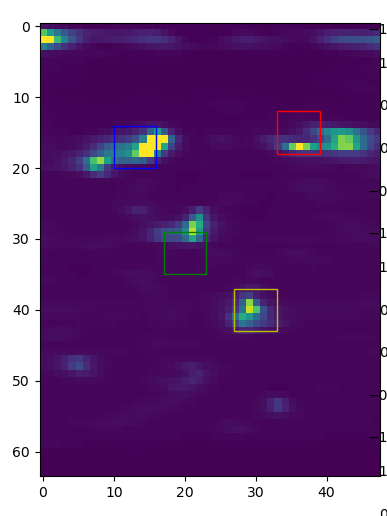
\includegraphics[width=.4\textwidth]{figures/validation/4personen_testen_crop.png}
    \caption{Four persons detected during the four person validation.}
    \label{fig:4_persons_detected}
\end{figure}

The graphs visualizing the measurement data for all four persons at the same time can be found in Figure~\ref{fig:4pers_heart_meas} and Figure~\ref{fig:4pers_breath_meas}. The most outstanding observation which can be done, is that the estimations from the IWR6843 are really jumping up and down. The measurements from the control measurement are much more stable. A positive observation is that the control measurement is most of the time approximately the average of the noisy measurements from the IWR6843. This is also confirmed with the numerical results in Table~\ref{tab:4pers_results} and Table~\ref{tab:4pers_results_2}. The numbers in this table are calculated in the same way as Section~\ref{sec:one_pers_validation}. In Table~\ref{tab:4pers_results}, each single result from the IWR6843 and the control measurement is compared to each other, which gives a large deviation because of the scattered results from the radar sensor. In Table~\ref{tab:4pers_results_2}, all measurements are averaged in one number. In this case, the deviation is much smaller.

The two person validation and the four person validation are also summarized in Bland-Altman plots. From these plots the mean difference between the two measurement types and the standard deviation can be observed. The multiple person heart rate Bland-Altman plot can be found in Figure~\ref{fig:ba_multiple_heart}, respiratory rate plot can be found in Figure~\ref{fig:ba_multiple_breath}.

\begin{table}[ht]
\centering
\begin{tabular}{|r|c|c|l|}
\hline
\textbf{Person} & \textbf{\begin{tabular}[c]{@{}c@{}}Heart rate\\ accuracy\end{tabular}} & \textbf{\begin{tabular}[c]{@{}c@{}}Respiratory\\ rate accuracy\end{tabular}} & \textbf{Average} \\ \hline
\textbf{P3} & 87.9\% & 78.5\% & \textbf{83.2\%} \\
\textbf{P10} & 78.8\% & 67.8\% & \textbf{73.3\%} \\
\textbf{P11} & 75.7\% & 74.8\% & \textbf{75.2\%} \\
\textbf{P12} & 81.9\% & 89.9\% & \textbf{85.9\%} \\ \hline
\textbf{Average} & \textbf{81.1\%} & \textbf{77.8\%} & \textbf{79.4\%} \\ \hline
\end{tabular}
\caption{Four person vital signs estimation validation results. The percentage denotes the absolute difference between the IWR6843 heart- and respiration rate, and the control rates.}
\label{tab:4pers_results}
\end{table}

\begin{table}[ht]
\centering
\begin{tabular}{|r|c|c|l|c|c|l|}
\hline
\textbf{Person} & \textbf{\begin{tabular}[c]{@{}c@{}}Heart rate\\ SpO2 \\ sensor\end{tabular}} & \textbf{\begin{tabular}[c]{@{}c@{}}Heart rate\\ IWR6843\end{tabular}} & \textbf{\begin{tabular}[c]{@{}l@{}}Heart rate\\ accuracy\end{tabular}} & \textbf{\begin{tabular}[c]{@{}c@{}}Respi-\\ ratory\\ rate\end{tabular}} & \textbf{\begin{tabular}[c]{@{}c@{}}Respi-\\ ratory\\ rate\\ IWR6843\end{tabular}} & \textbf{\begin{tabular}[c]{@{}l@{}}Respi-\\ ratory\\ rate\\ accuracy\end{tabular}} \\ \hline
\textbf{P3} & 61 & 64 & \textbf{94.4\%} & 7 & 9 & \textbf{71.8\%} \\
\textbf{P10} & 66 & 63 & \textbf{95.0\%} & 10 & 9 & \textbf{94.0\%} \\
\textbf{P11} & 69 & 58 & \textbf{83.9\%} & 8 & 9 & \textbf{97.6\%} \\
\textbf{P12} & 69 & 60 & \textbf{87.1\%} & 11 & 11 & \textbf{97.9\%} \\ \hline
\textbf{Average} &  &  & \textbf{90.1\%} &  &  & \textbf{90.3\%} \\ \hline
\end{tabular}
\caption{Four person vital signs estimation validation results. The average heart rates and respiratory rates of all sensors from the whole reading, with the accuracy between the control measurements and the IWR6843 measurements.}
\label{tab:4pers_results_2}
\end{table}

\begin{figure}[t]
\centering
\begin{subfigure}{.45\textwidth}
  \centering
  % include first image
  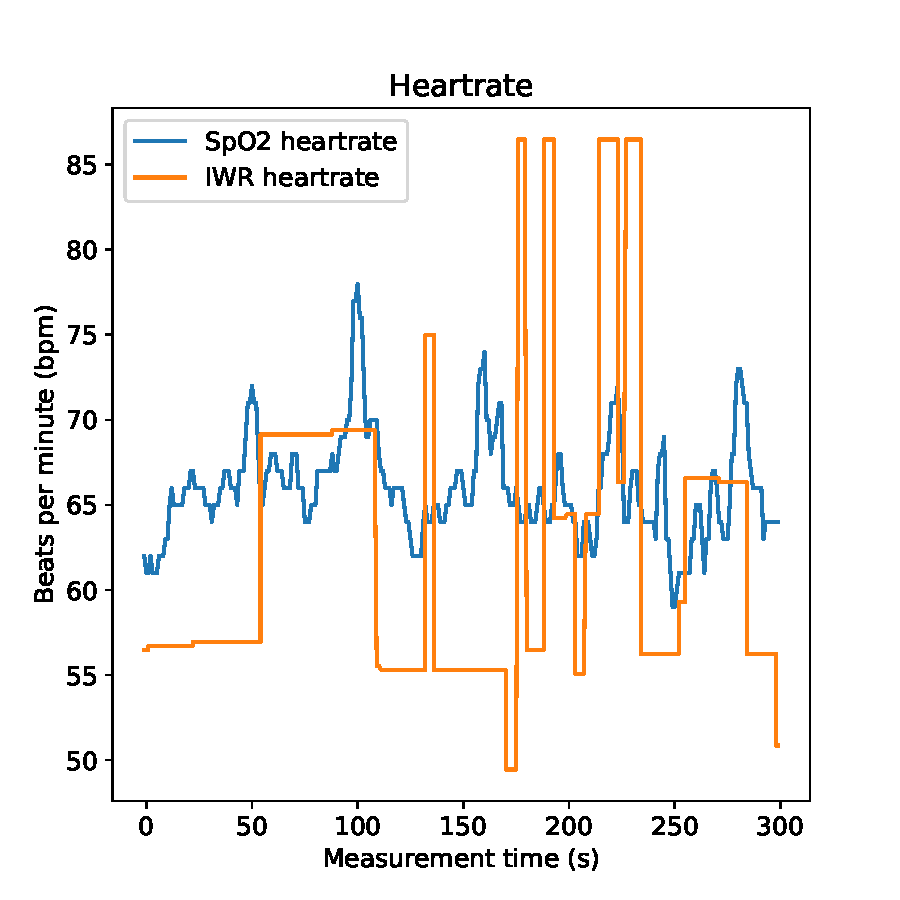
\includegraphics[width=\linewidth]{figures/validation/roy4_heart.pdf}  
  \caption{heart rate of \emph{P3}}
  \label{fig:roy4_heart}
\end{subfigure}
\begin{subfigure}{.45\textwidth}
  \centering
  % include second image
  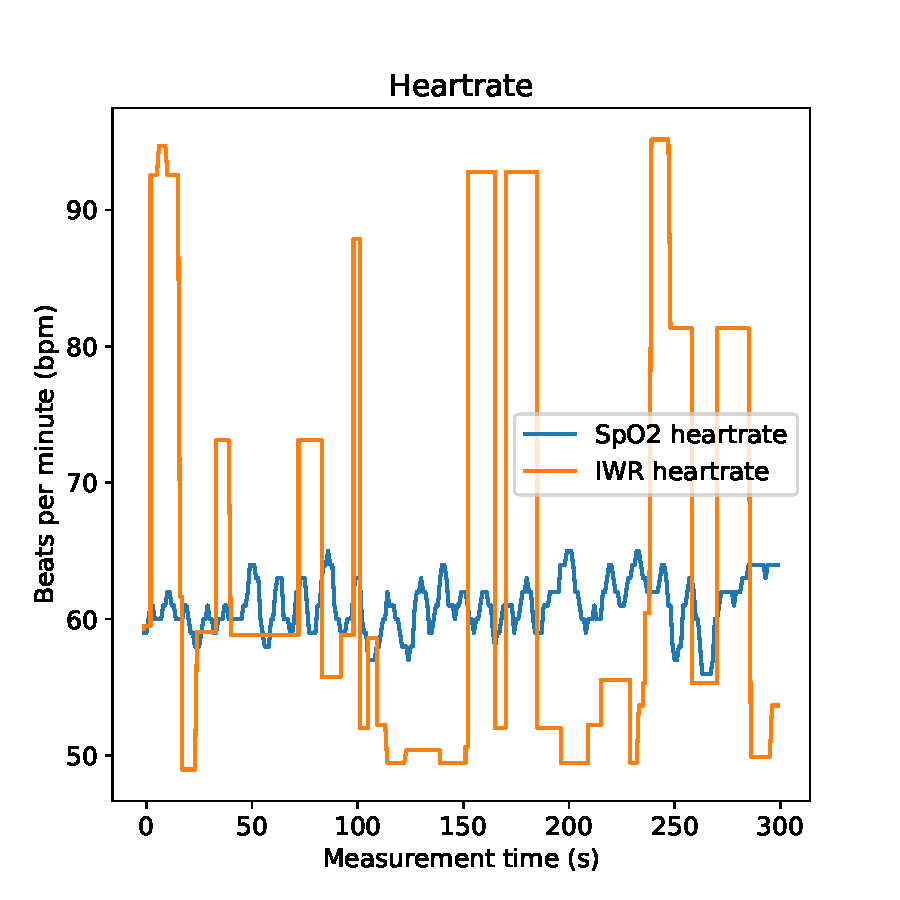
\includegraphics[width=\linewidth]{figures/validation/nick4_heart.pdf}  
  \caption{heart rate of \emph{P10}}
  \label{fig:nick4_heart}
\end{subfigure}
\begin{subfigure}{.45\textwidth}
  \centering
  % include third image
  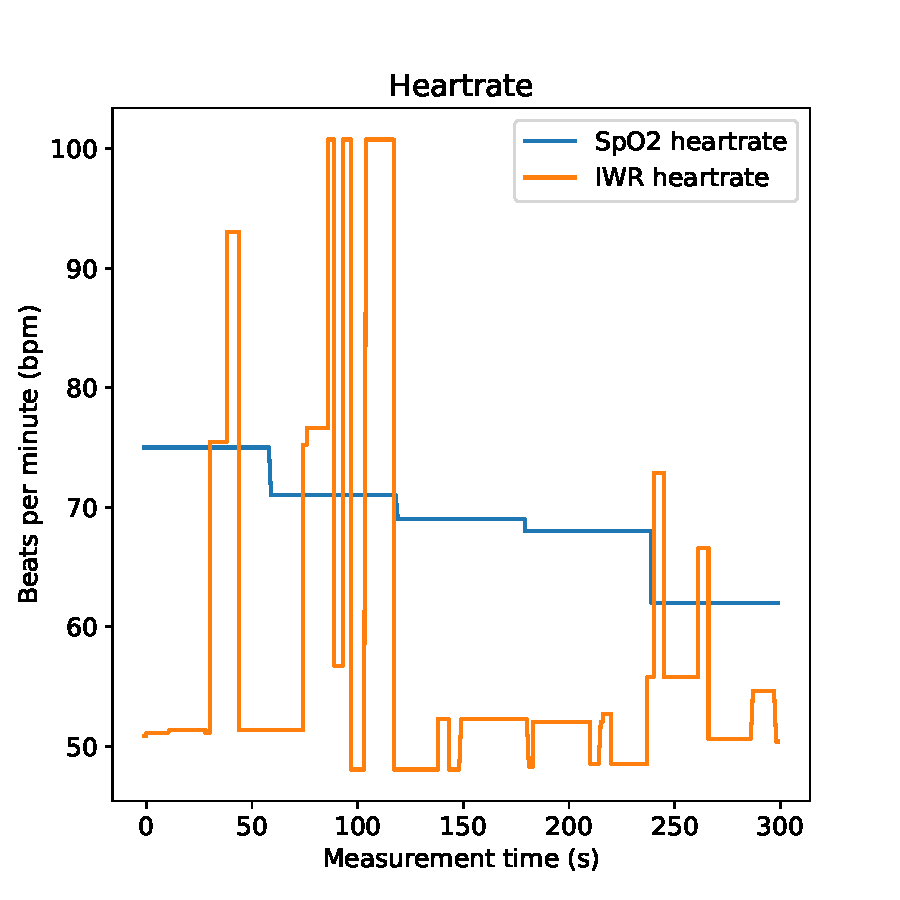
\includegraphics[width=\linewidth]{figures/validation/pascal4_heart.pdf}  
  \caption{heart rate of \emph{P11}}
  \label{fig:pascal4_heart}
\end{subfigure}
\begin{subfigure}{.45\textwidth}
  \centering
  % include fourth image
  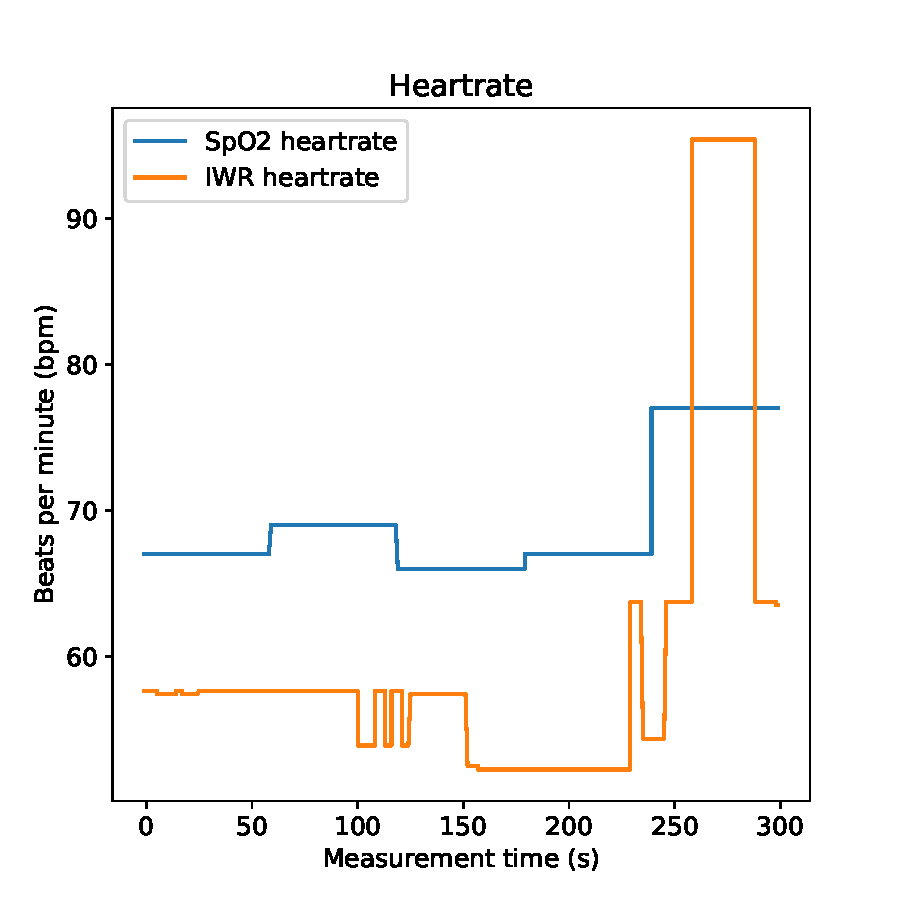
\includegraphics[width=\linewidth]{figures/validation/romy4_heart.pdf}  
  \caption{heart rate of \emph{P12}}
  \label{fig:romy4_heart}
\end{subfigure}
\caption{heart rate estimation from 4 persons at the same time.}
\label{fig:4pers_heart_meas}
\end{figure}

\begin{figure}[t]
\centering
\begin{subfigure}{.45\textwidth}
  \centering
  % include first image
  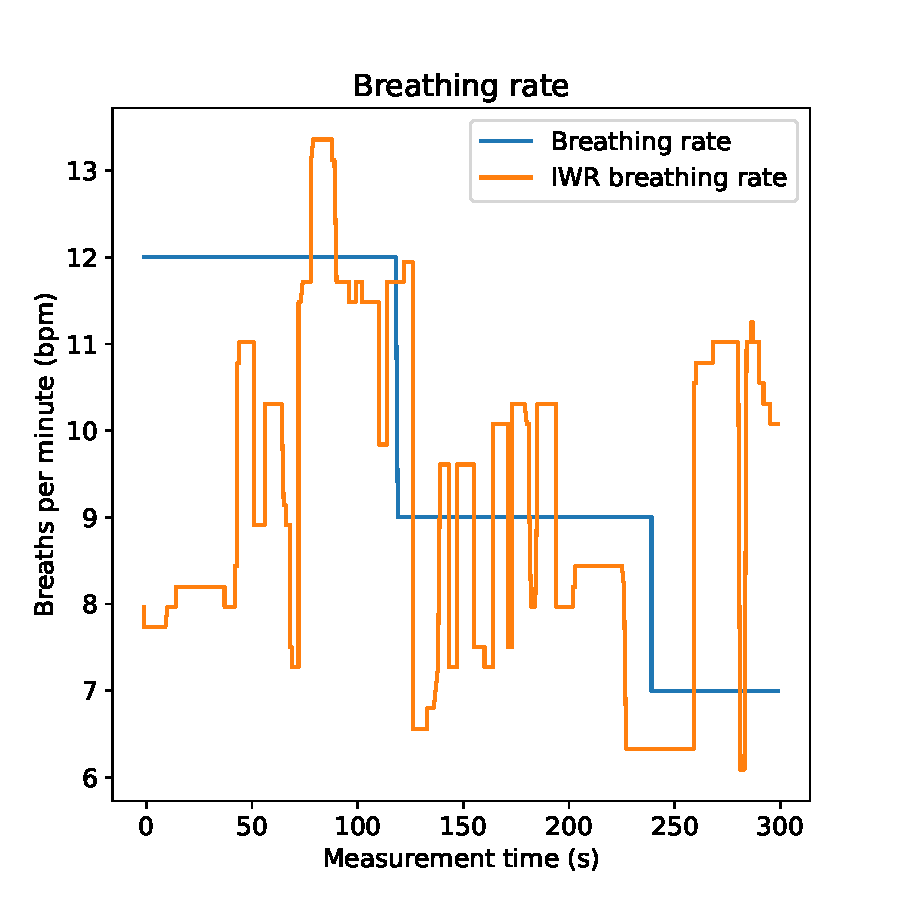
\includegraphics[width=\linewidth]{figures/validation/roy4_breath.pdf}  
  \caption{Respiratory rate of \emph{P3}}
  \label{fig:roy4_breath}
\end{subfigure}
\begin{subfigure}{.45\textwidth}
  \centering
  % include second image
  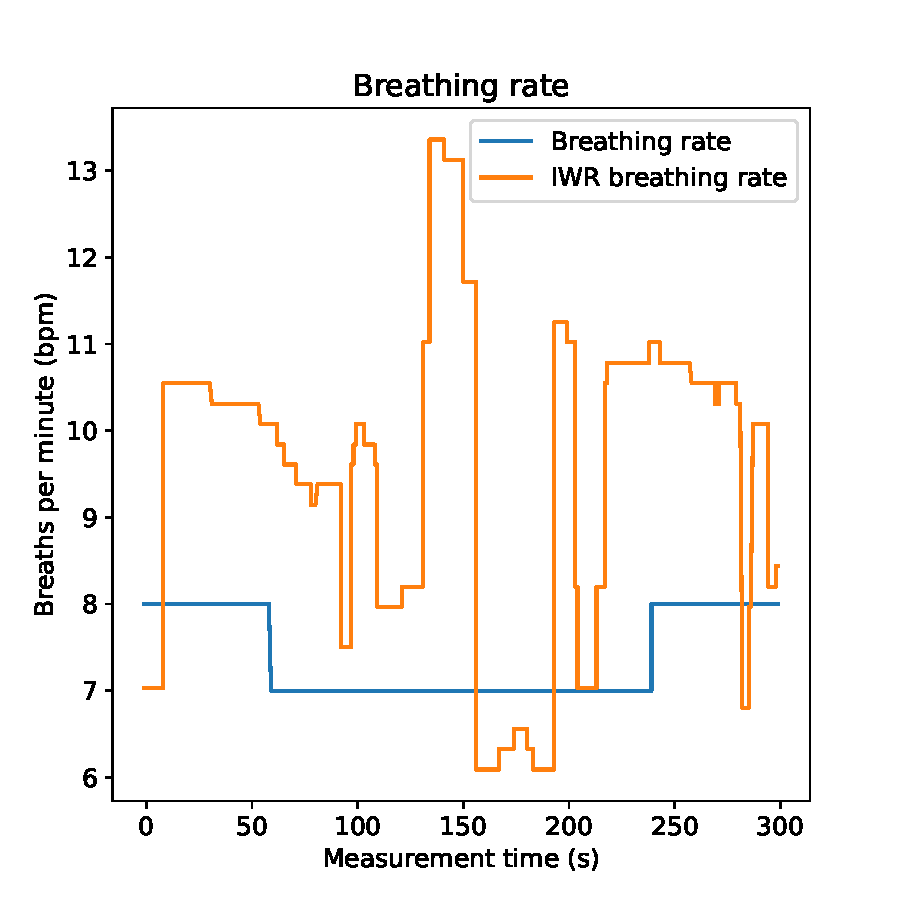
\includegraphics[width=\linewidth]{figures/validation/nick4_breath.pdf}  
  \caption{Respiratory rate of \emph{P10}}
  \label{fig:nick4_breath}
\end{subfigure}
\begin{subfigure}{.45\textwidth}
  \centering
  % include third image
  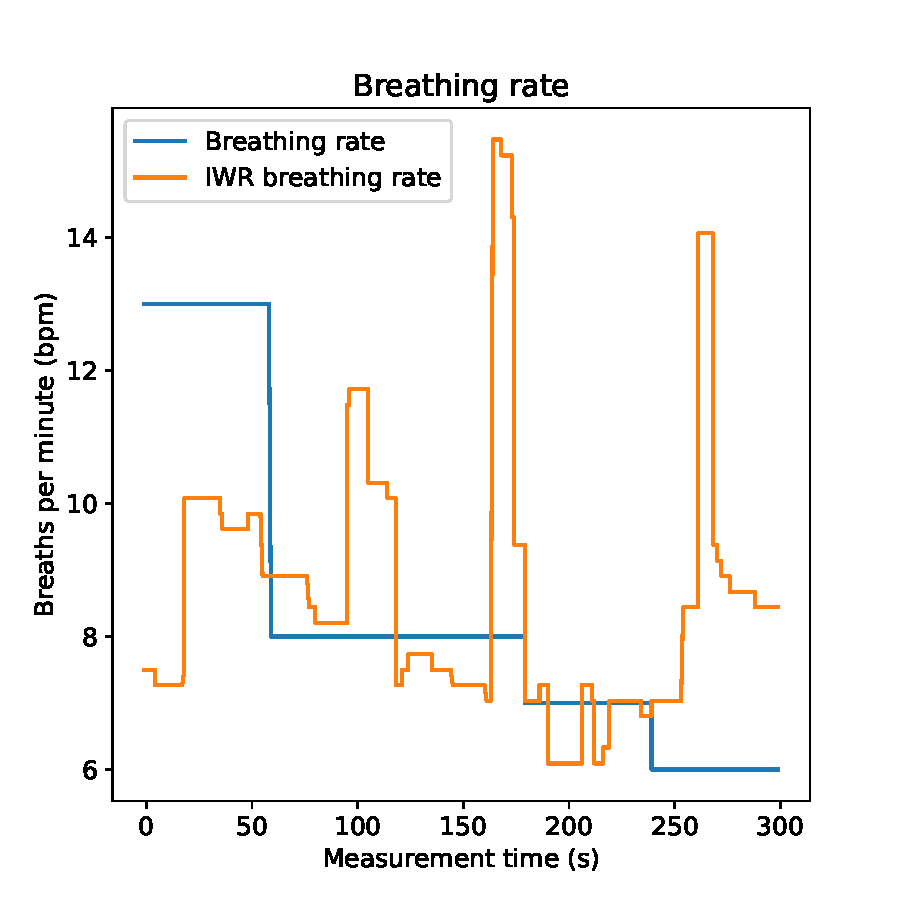
\includegraphics[width=\linewidth]{figures/validation/pascal4_breath.pdf}  
  \caption{Respiratory rate of \emph{P11}}
  \label{fig:pascal4_breath}
\end{subfigure}
\begin{subfigure}{.45\textwidth}
  \centering
  % include fourth image
  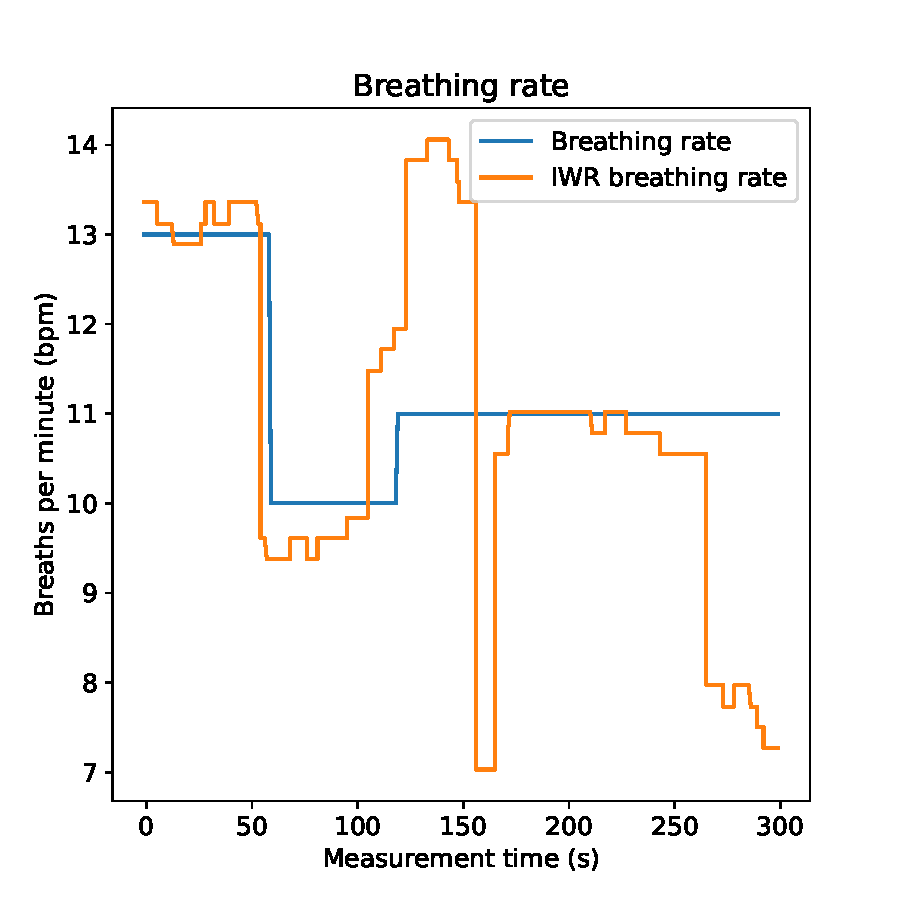
\includegraphics[width=\linewidth]{figures/validation/romy4_breath.pdf}  
  \caption{Respiratory rate of \emph{P12}}
  \label{fig:romy4_breath}
\end{subfigure}
\caption{Respiratory rate estimation from 4 persons at the same time.}
\label{fig:4pers_breath_meas}
\end{figure}

\begin{figure}[t]
    \centering
    \hspace*{-2cm}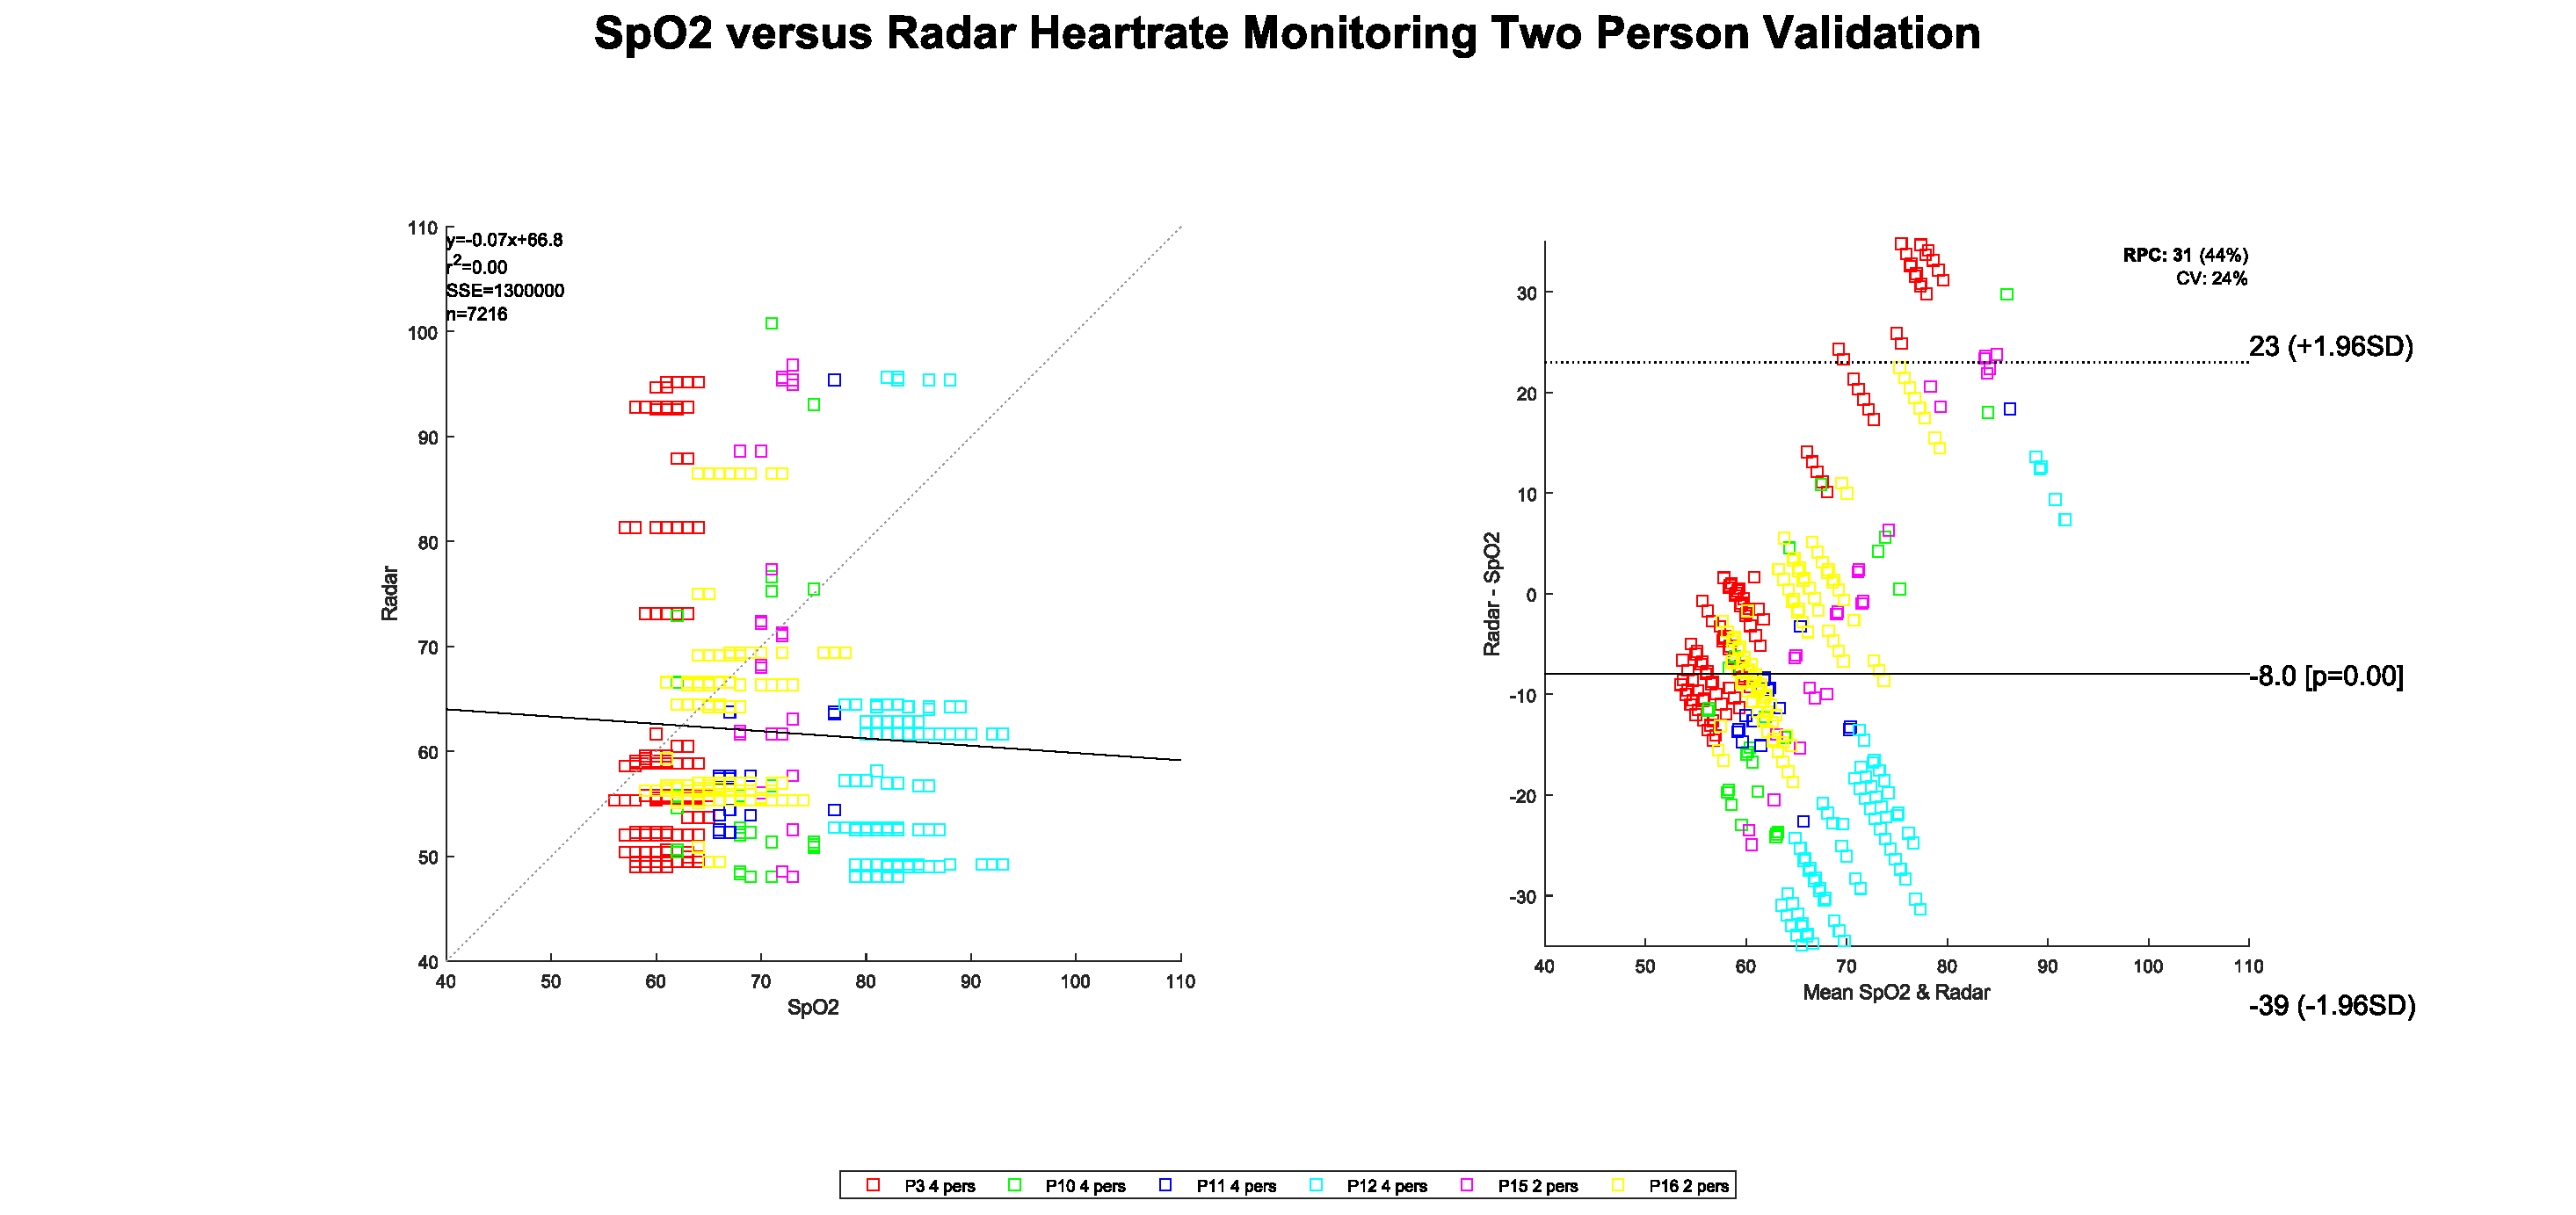
\includegraphics[width=1.2\textwidth]{figures/validation/bland_altman_multiple.pdf}
    \caption{Bland-Altman plot of all multiple person heart rate validation results.}
    \label{fig:ba_multiple_heart}
\end{figure}

\begin{figure}[t]
    \centering
    \hspace*{-2cm}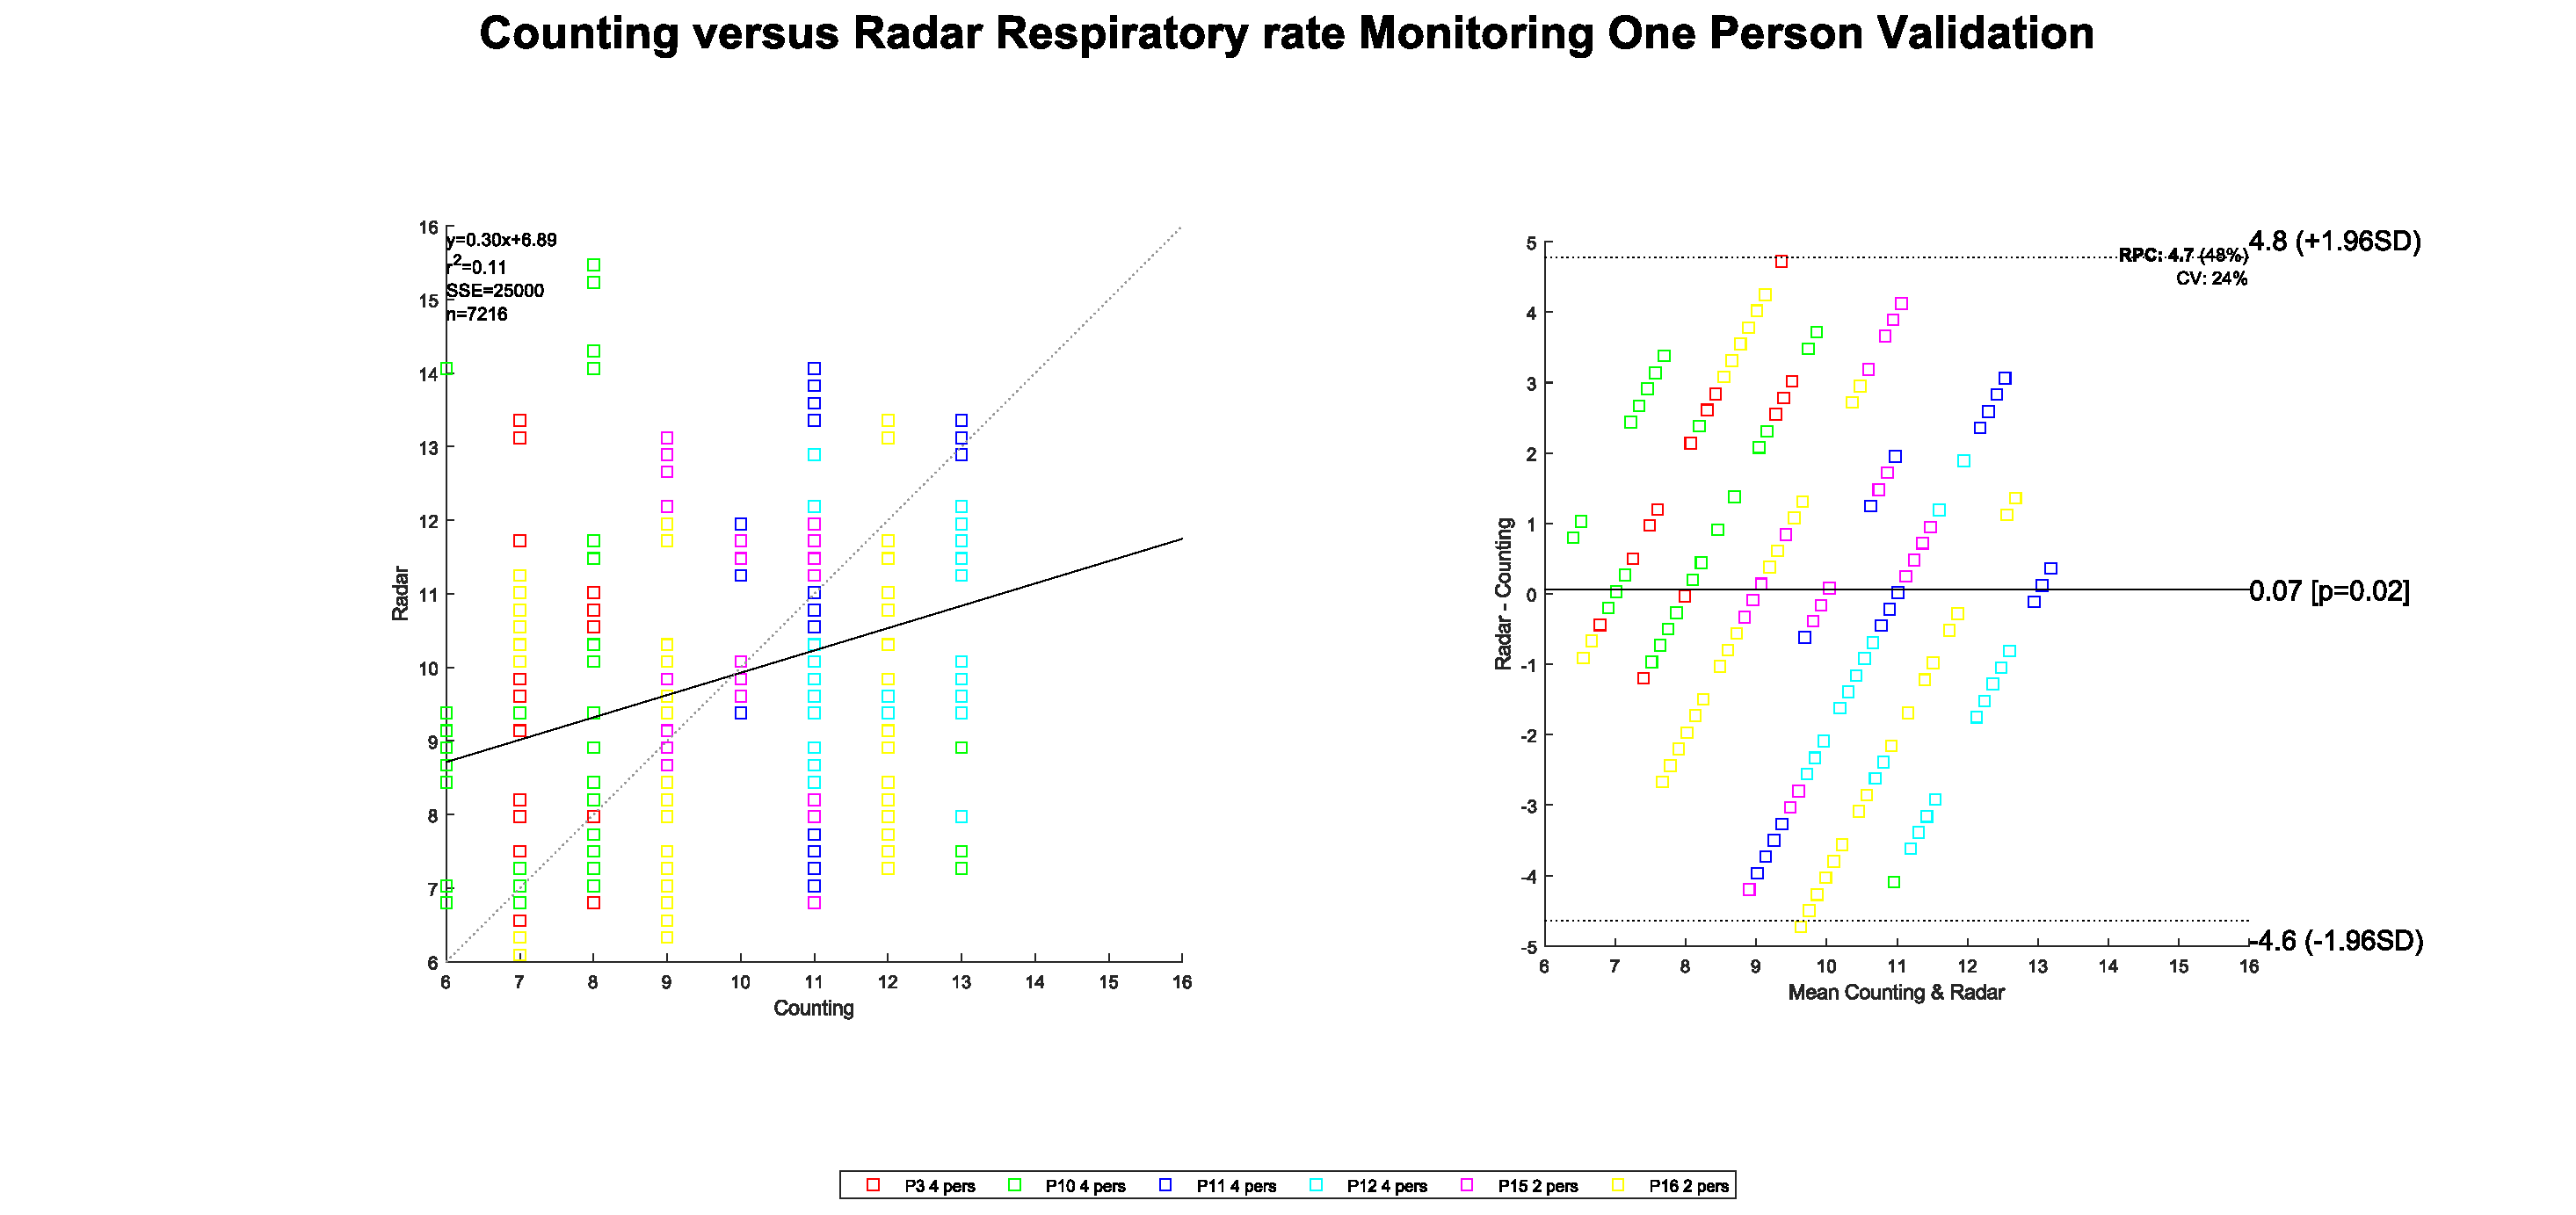
\includegraphics[width=1.2\textwidth]{figures/validation/bland_altman_multiple_BR.pdf}
    \caption{Bland-Altman plot of all multiple person respiratory rate validation results.}
    \label{fig:ba_multiple_breath}
\end{figure}

\subsection{mmWave radar accuracy compared to test subject variables}
When performing the validation tests, some variables from the test subjects were captured, see also Section~\ref{sec:person_metrics}. An interesting observation would be to see if there is a correlation between those variables and the measurement accuracy. This would make sure that vital signs monitoring using mmWave radar would be a viable option for all types of persons. The accuracy is compared against the age, BMI and sex of a person. The age and BMI graphs can be observed in Figure~\ref{fig:age_bmi_corr}.

\subsubsection{Age}
In Figure~\ref{fig:age_corr} the mean difference between the radar measurement and the control measurement is plotted against the age of the test subject. In this graph, no correlation can be observed. This means that the age of a person has nothing to do with the accuracy of the vital signs estimation.

\subsubsection{Weight / BMI}
\label{sec:weight_res}
In Figure~\ref{fig:bmi_corr}, the BMI of a test subject is plotted against the mean difference between the radar vital signs estimation and the control measurement. The BMI variable has been chosen, because persons with a higher BMI generally also have more fat in their body. The hypothesis is that this fat could dampen the vibrations from which the vital signs are deduced. Again, no clear correlation can be found between this metric and the variable. This means that this type of measurement could be used for bigger persons, but also for more skinny persons.

\begin{figure}[t]
\centering
\begin{subfigure}{.45\textwidth}
  \centering
  % include first image
  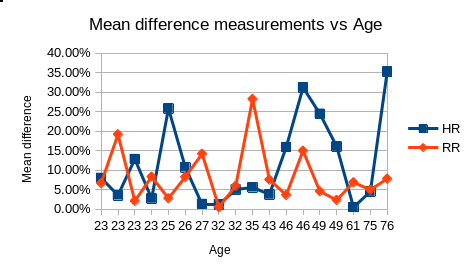
\includegraphics[width=\linewidth]{figures/validation/age_correlation.png}  
  \caption{Correlation between the mean difference of the measurements and the age of the test subject.}
  \label{fig:age_corr}
\end{subfigure}
\begin{subfigure}{.45\textwidth}
  \centering
  % include second image
  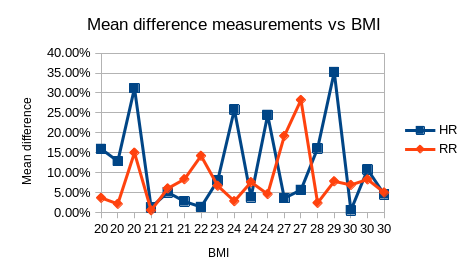
\includegraphics[width=\linewidth]{figures/validation/bmi_correlation.png}  
  \caption{Correlation between the mean difference of the measurements and the age of the test subject.}
  \label{fig:bmi_corr}
\end{subfigure}
\caption{Correlation between the mean difference of the measurements and two test subject variables.}
\label{fig:age_bmi_corr}
\end{figure}

\subsubsection{Sex}
The mean difference between the radar estimation and the control measurement for female test subject's heart rate is 8.74\%, for the respiratory rate it is 4.42\%. The mean difference for the male test subject's heart rate is 11.76\%, the respiratory rate difference is 9.04\%. The difference between the measurements for the male test subjects is higher, but not by a large amount. This difference could also be due to measurement inaccuracies. Because the validation was performed on only 4 female test subjects compared to 12 male test subjects, more female validations need to be done to come up with a definite conclusion.
% \todo{Conclusion?}

\section{Evaluation}
When observing the result from the one person-, two person- and four person validation, it could be noted that the accuracy reduces when there are more persons in the sensor view. This could have multiple reasons. Because there are more persons in the field of view of the radar, more noise is introduced. The test subjects all constantly move very slightly, this could introduce noise in the very sensitive phase information. Another option could be that the phase changes of the different persons interfere with each other. More knowledge about radar theory could probably substantiate that hypothesis.

Taking into account all of the measurements from the 16 test subjects in the different configurations, this gives a good representation of the accuracy of the prototype of this project. The algorithms could be tuned better to make the sensor measurements more stable and generally more accurate, but the main goal of this project is to see if the algorithms can be put on the sensor chip itself, and if it would hold up against the large stream of radar data which was coming in. This goal has been reached, because the sensor never missed a timing deadline during the validation phase.